\documentclass[a4paper,11pt,titlepage]{jsarticle}

\usepackage{amsmath}
\usepackage{amssymb}
\usepackage{amsfonts}
\usepackage{bm}
\usepackage[dvipdfmx]{graphicx}
\usepackage{listings}
% \usepackage{jvlisting}
% \usepackage{jlisting}
\usepackage{otf}
\usepackage{float}
\usepackage{url}
\usepackage{ascmac}
\usepackage{fancybx}
\usepackage{subcaption}
\usepackage{caption}
\usepackage[margin=1in]{geometry} % ページ余白を狭めて表示領域を広く

% \bibliographystyle{junsrt} % スタイル(番号順)
% \bibliographystyle{plain}
% \bibliography{references}  % references.bib を指定(拡張子は不要)

\lstset{%ソースコードの表示に関する設定
    basicstyle={\ttfamily},
    identifierstyle={\small},
    commentstyle={\smallitshape},
    keywordstyle={\small\bfseries},
    ndkeywordstyle={\small},
    stringstyle={\small\ttfamily},
    frame={tb},
    breaklines=true,
    columns=[l]{fullflexible},
    numbers=left,
    xrightmargin=0zw,
    xleftmargin=3zw,
    numberstyle={\scriptsize},
    stepnumber=1,
    numbersep=1zw,
    lineskip=-0.5ex
}

% 画像ファイルを検索するディレクトリを指定
\graphicspath{ {images/} }
%これを設定しておけば,自動的にimages/から画像を参照してくれる。
%================================

\begin{document}

\title{知能情報実験 \ajroman{3}(データマイニング班) \\ 顔画像に基づく美男美女と一般人との比較による特徴抽出}
\author{215706D:KIM HYUNWOO, 235221E:山脇大輝,\\ 235701B:松田遼平, 235732B:長\UTF{7028}一生}
\date{提出日: 2025年7月18日}
\maketitle

\tableofcontents
\clearpage

\begin{abstract}
\label{label:abstract}
本研究では,FairFaceデータセットを一般人データとして用い,独自に構築した美男美女データセットと併せて学習を行うことで,人物の外見に基づく分類を行う機械学習システムを構築した。さらに,Grad-CAMを用いて各モデルの判断根拠を可視化し,信頼性の評価を試みた。
追加学習を行ったFairFaceモデルにおいては,顔領域を適切に着目しながら一般人・美男美女の分類精度100\%を達成したが,新規学習したResNet18,ResNet34,ResNet50,EfficientNet\_b0については,分類精度95\%を超える高い分類精度を示したものの顔ではなく画像の背景を見ていることが確認された。ここからデータセット構築時における内在的バイアスが含まれていることがわかった。深層学習モデルが高精度を示す場合でも,その判断根拠が実験目的と合致しているとは限らないという,モデルの信頼性における重要な課題を浮き彫りにした。
また,Custom ModelではGradCamの結果より目元と口元を見て一般人と美男美女を分類していることから,これらが一般人と美男美女の差異であると結論付けた。
\end{abstract} 


\section{はじめに}
\label{label:はじめに}
\subsection{実験の目的と達成目標(アプローチの全体像を含む)}
本グループでは「顔画像データを用いて,一般的に“美男美女”と称される有名人と一般人を識別・分類し,特徴差を明らかにすること」をテーマとして設定した。

人の美しさや魅力は主観的に表されることが多く,機械学習を用いて客観的に分析することを試みる。FairFaceのモデル構築の際に用いられた画像群と独自に美男美女の画像から構築したデータセットを用いて,画像認識のための深層学習モデルであるResNet18, ResNet34, ResNet50とEfficientNet\_b0を用いて,美男美女(有名人)と称される顔写真と一般人の写真を識別・分類するモデルの構築を問題として設定した。最終的には,GradCamを用いて実行結果を可視化し,美男美女と一般人の顔写真を区別する上で重要になる特徴を定量的に見る。
%最終的には,美男美女と一般人の差から美しさや魅力度合いがどのように違うのかを定量化・可視化し,美的評価の要素を客観的に明らかにする。
%また,人の美しさは黄金比や対称性といった要素で評価されることが多いが,モデルが人間の美的感覚に近い判断をどの程度行えるかというデータを明らかにする.

\subsection{意図していた実験計画との違い}
\label{label:意図していた実験計画との違い}
当初の調査段階では,FairFaceがデータセットのみを公開していると認識していたが,実際には高精度な学習済みモデル(ResNet-34ベース)も提供されていることが後に判明した。FairFaceと同様のデータセット構築とモデル学習を一から行うことは,実験としての新規性が少ない。そこで,方針を転換しFairFaceの学習済みモデルに対して,独自に収集した美男美女・一般人のラベル付をした画像を学習させることで追加学習を行うアプローチを行うことにした。

\subsection{実験の全体像}
%======================
\begin{figure}[H]
    \centering
    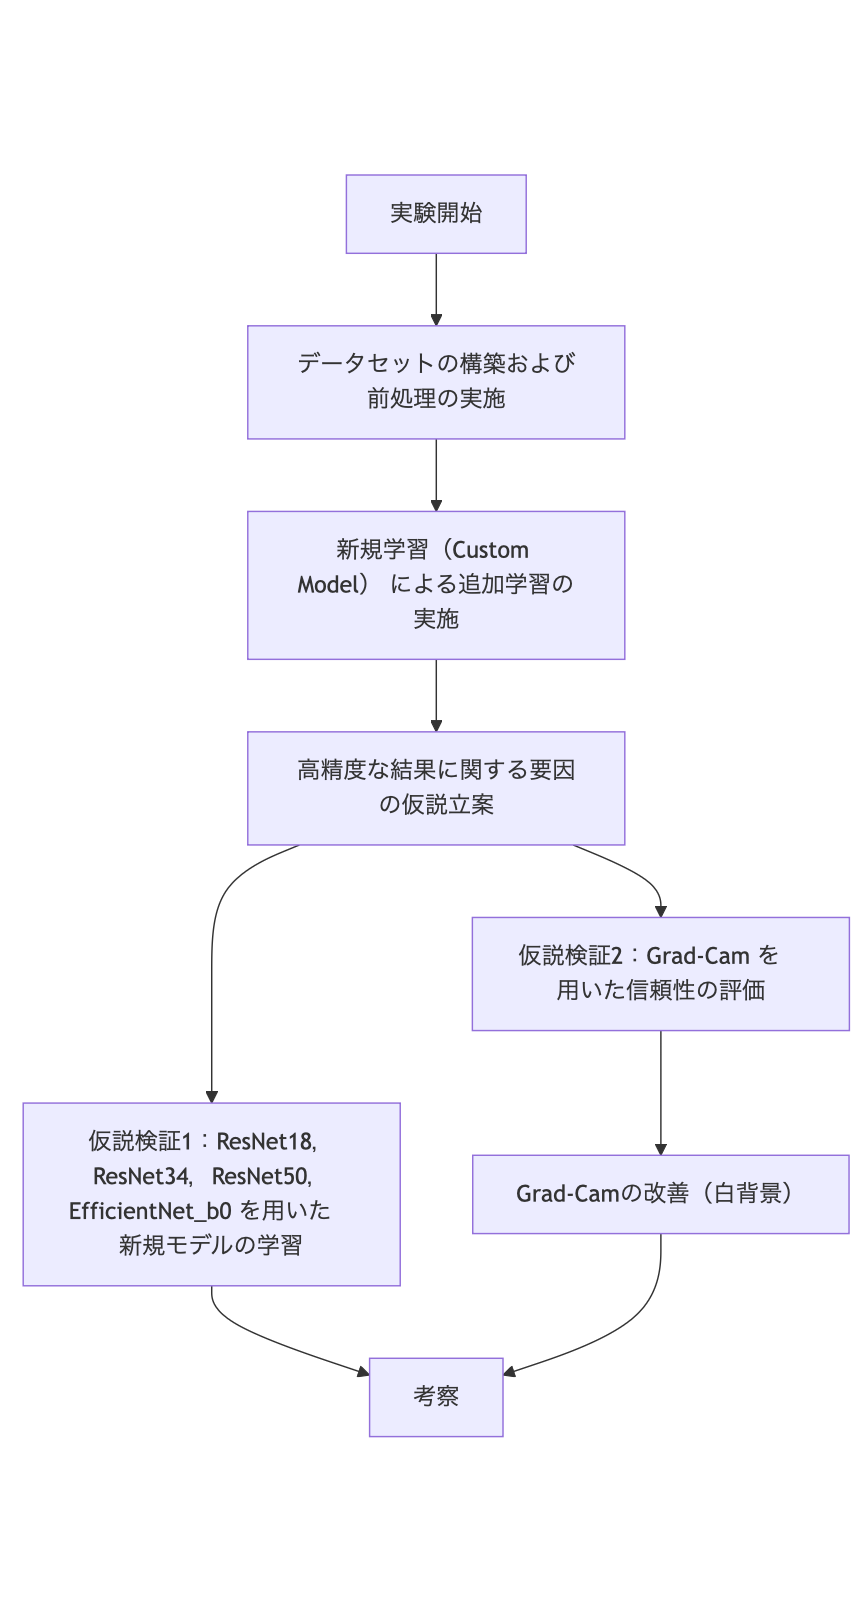
\includegraphics[width=100mm]{overall.png}
    \caption{実験のフローチャート}
    \label{fig:csv}
\end{figure}
%======================

\section{実験方法}
\label{label:実験方法}
\subsection{実験目的}
世界で美男美女と呼ばれる人の顔写真と一般人の顔写真を分類するモデルを作り,美男美女と一般人の分類を行う。

\subsection{データセット構築・前処理}
美男美女と一般人を分類するモデルを構築するために,2つのデータセットを準備し,前処理を行い,モデルの学習・評価を行う。
前処理のフローチャートを図\ref{fig:prepro}に示す。


\subsubsection{FairFaceとは}
本実験ではFairFaceというモデルを用いて,分類評価を行うと同時に,独自構築した分類モデルも作成した。ここで,FairFaceというモデルについて概要を説明すると,従来の多くの顔画像データセットでは,特定の人種(白人)や性別にデータの偏りが見られる傾向にある。FairFaceでは,7つの人種グループ:白人,黒人,インド人,東アジア人,東南アジア人,中東人,ラテンアメリカ人でデータ数を均一して,人種差の少ないデータセット構築を行った。この論文の実験では,FairFaceデータセットを含む様々なデータセットでモデルを訓練し,その後に訓練されたモデルを用いて新しいデータセットでの汎化性能を評価しており,機械学習モデルの特定の人種・性別への偏り・バイアスの軽減を実現した顔画像データセット及びモデルである。
構築されたデータセットについては,主に大規模なパブリックデータセットyahoo YFCC100M(Flickr画像)から,意図的に人種バランスを考慮したサンプリング手法を用いて収集され,加えてTwitterやオンライン新聞からの画像も含まれている。YFCC100M全体からランダムに顔画像をサンプリングし,各国の人口構成を推定し,データセットが特定(白人)の人種に偏らないように画像数を調節した。これにより他の人種を過小評価するデータセットのバイアスを軽減している。




\subsubsection{定義}
本実験では,以下のように一般人と美男美女の定義を行う。
\begin{itemize}
    \item 一般人:FairFaceのデータセットで作成されたデータセット。
    \item 美男美女:2024年度世界の美男美女ランキング上位top50を美男美女として定義する。
\end{itemize}

\subsubsection{データセット構築}
\begin{itemize}
    \item 一般人のデータセット:FairFaceのデータセットを使用
    \item 美男美女のデータセット:独自構築を行った。
        \begin{itemize}
            \item[(1)] 美男美女の基準を決定 \\
                文献\cite{bidanshi}や文献\cite{bijoshi}より2024年度美男美女ランキングtop50を美男美女として扱う
            \item[(2)] データの収集 \\
                対象者の画像は,「2024年度美男美女ランキング」top50の人名からbing検索エンジンを用いてwebスクレイピングした。
                \begin{itemize}
                	\item	人名でキーワード検索を行い,人物以外のもの(例えば似顔絵やファングッズなど)を除外した。(いわゆる宣材写真のみ収集したわけではない。)
                    \item ソースコードを以下のGitHubにて公開する。
                    \item \url{https://github.com/e235221/info3dm_racial_classification}
                \end{itemize}
        \end{itemize}
\end{itemize}
    
\subsubsection{前処理}
\begin{itemize}
    \item リサイズ
        \begin{itemize}
            \item 収集したデータの顔部分だけ切り取り,サイズを$300 \times 300$とし,FairFaceのデータセットと合わせて調整する.
        \end{itemize}
    \item 正面・側面の判定
        \begin{itemize}
            \item 顔の向きが学習に与える影響を排除するために,hopenetを用いて正面を向いている画像のみ抽出した。側面を向いている画像はデータセットから除外している。
            \item HopeNetとは,1枚の顔写真からYaw(左右の向き),Pitch(上下の向き),Roll(傾き)を求め,その人がどの方向を向いているのかを推定する深層学習モデルである。感情認識などに用いられている。
        \end{itemize}
    \item アップサンプリング・ダウンサンプリング
        \begin{itemize}
            \item アップサンプリング:データ数の少ない美男美女データの各画像を左右反転させることでデータ数を2倍に増やした。
            \item ダウンサンプリング:データ数の多い美男美女データセットからランダムにデータを削除することで,美男美女データセットと一般人データセットのデータ件数を調節した。
            \item 画像数については,trainで31000枚ずつ,testで7800枚ずつの画像を用意した。
        \end{itemize}
    \item 美男美女・一般人データセットに対して,ラベル付け
        \begin{itemize}
            \item webスクレイピングしで収集した画像データに対して,FairFaceで用意されているラベル付けと同様に美男美女データセットに対してもラベル付けを行い,それに加えて一般人か美男美女かを判別するためにそれぞれ0と1を付与した。
            \item 新規作成した美男美女データセットについては,手作業で検索し,国籍・誕生日のラベルを付与した。
            \item \texttt{file\_name,age,gender,race,0/1}の5種類を列名としてcsvを作成した。\texttt{file\_name}に指定されたpathで画像を読み込み,学習を行う。
        \end{itemize}
    \item ファイルのリネーム
\end{itemize}


\subsection{モデル選定}
FairFaceが提供する学習済みモデルを本研究のタスクに合わせてカスタマイズした。これにはResNet34が使用されていたため,そのままResNet34を用いる。詳しくは文献\cite{karkkainenFairFace}を参照されたい。\par
(後述するが,このFairFaceのカスタマイズモデルは精度が100\%になったため,別アプローチとして本実験ではFairFaceを用いず新規にResNet18, ResNet34, ResNet50も用いた。パラメータ調整はデフォルトのままである。)


\subsection{パラメータ調整}
本実験ではFairFaceのソースコードをパラメータ調整せずに使用した。
GitHubに公開されているFairFaceのソースコードでは,ハイパーパラメータが不明であるが,文献\cite{karkkainenFairFace}より学習率0.0001のOptimizerにADAM最適化が用いられている。ただしこれらのハイパーパラメータが選ばれた理由はGitHubや論文を読んでも不明である。
% 学習率は0.0001で,ADAM最適化を行っている。


%======================
\begin{figure}[H]
    \centering
    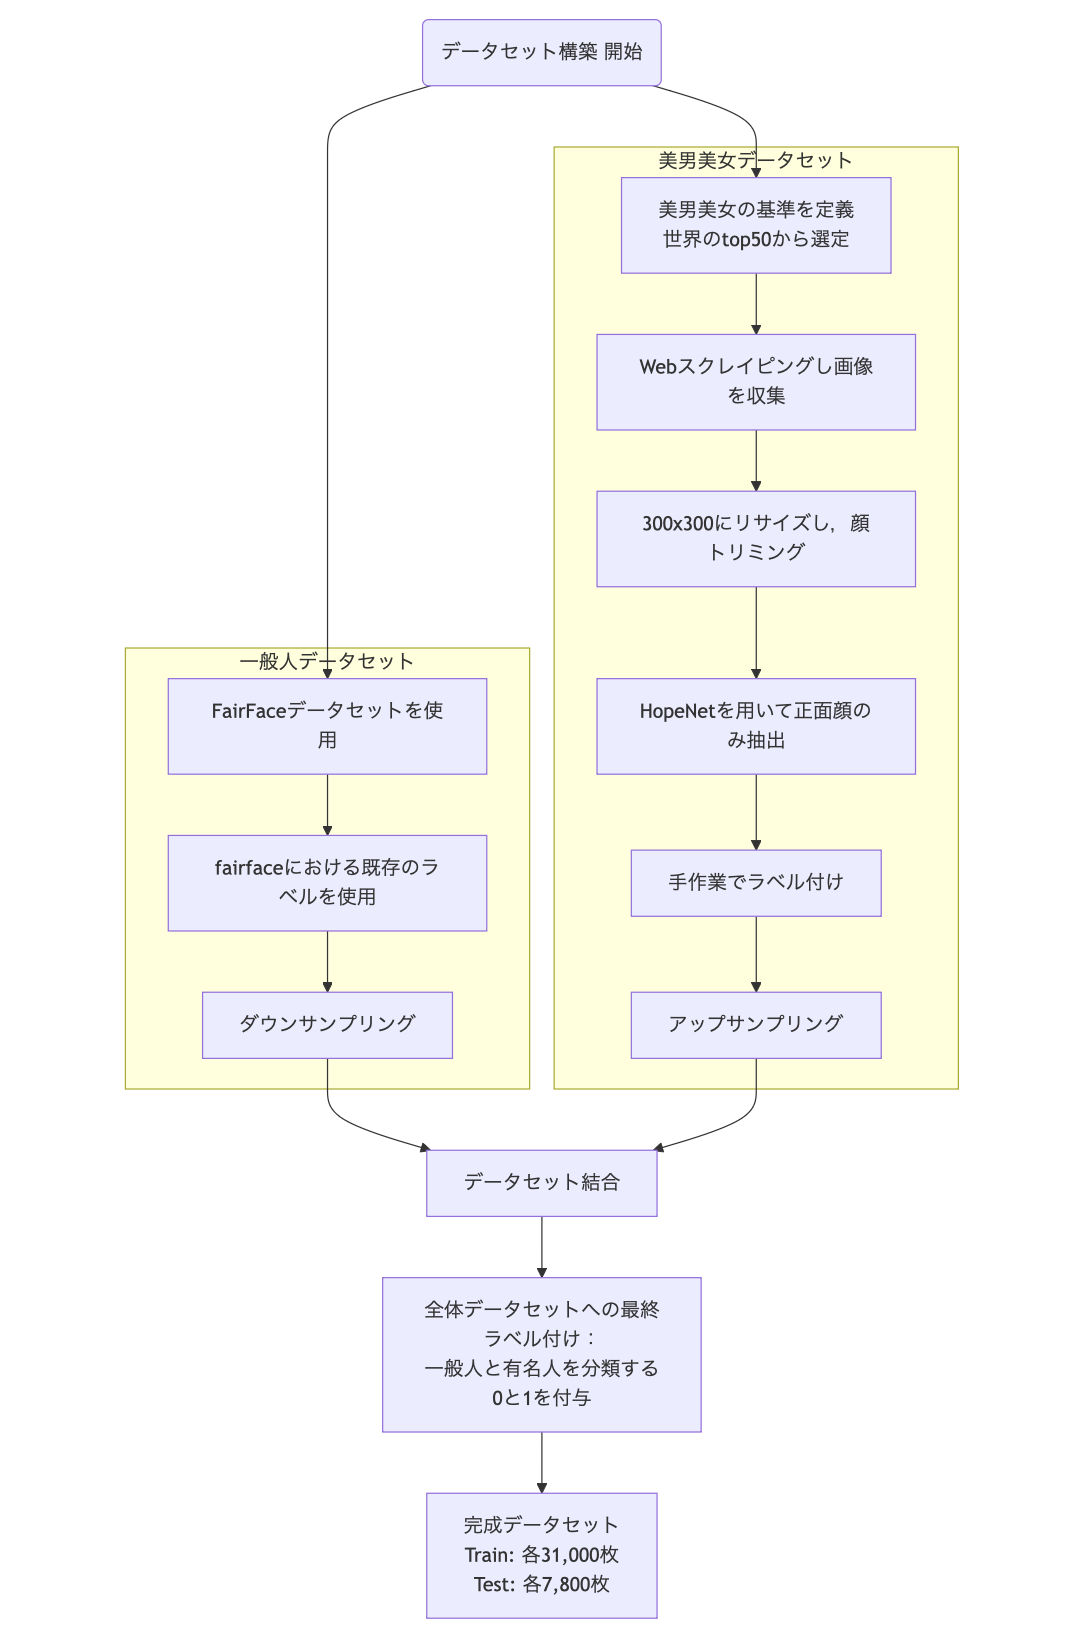
\includegraphics[width=0.9\textwidth]{preprocessing.png}
    \caption{前処理のフローチャート}
    \label{fig:prepro}
\end{figure}
%======================




\section{実験}
\label{実験}

\subsection{役割分担について}
\begin{itemize}
    \item 215706D:KIM HYUNWOO
        \begin{itemize}
            \item 正面画像抽出・ラベル付・複数のResNetとEfficientNetでの実行・Grad Cam
        \end{itemize}
    \item 235221E:山脇大輝
        \begin{itemize}
            \item FairFaceの調査,カスタマイズ,Webスクレイピング・リサイズ・トリミング・ラベル付
        \end{itemize}
    \item 235701B:松田遼平
        \begin{itemize}
            \item GitHubの操作補助
        \end{itemize}
    \item 235732B:長\UTF{7028}一生
        \begin{itemize}
            \item アップサンプリング・ダウンサンプリングコード作・背景のマスキング実施
        \end{itemize}
\end{itemize}

%\subsection{実験設計}
%\begin{itemize}
%    \item 実験の目標
%    \item 目標をどのように達成しようとしたのか
%\end{itemize}


\subsection{用意したデータセット画像}
図\ref{fig:good_ex},図\ref{fig:normal_ex}に用意したデータセットの画像の一部を示す。これは筆者がランダムに選択したものであり,レポートの可読性を向上させるために用意した。
%======================
\begin{figure}[htbp]
    \centering
    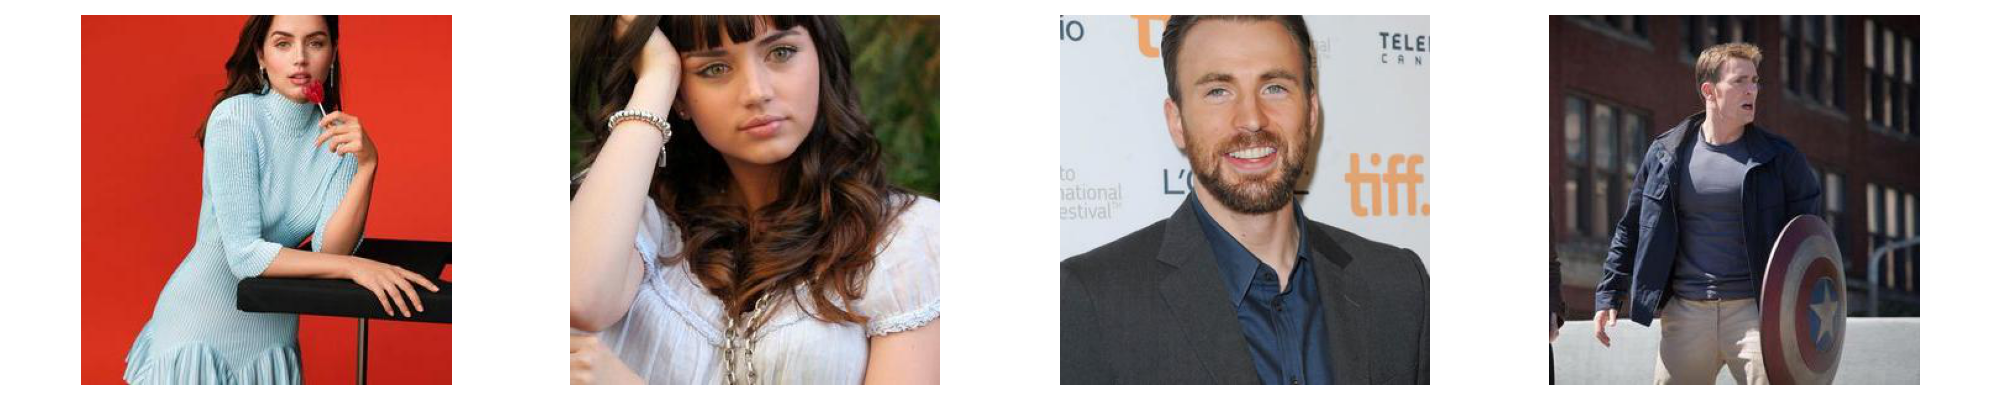
\includegraphics[width=1.1\textwidth]{ex_good_dataset.png}
    \caption{美男美女データセットの画像例}
    \label{fig:good_ex}
\end{figure}
%======================
%======================
\begin{figure}[H]
    \centering
    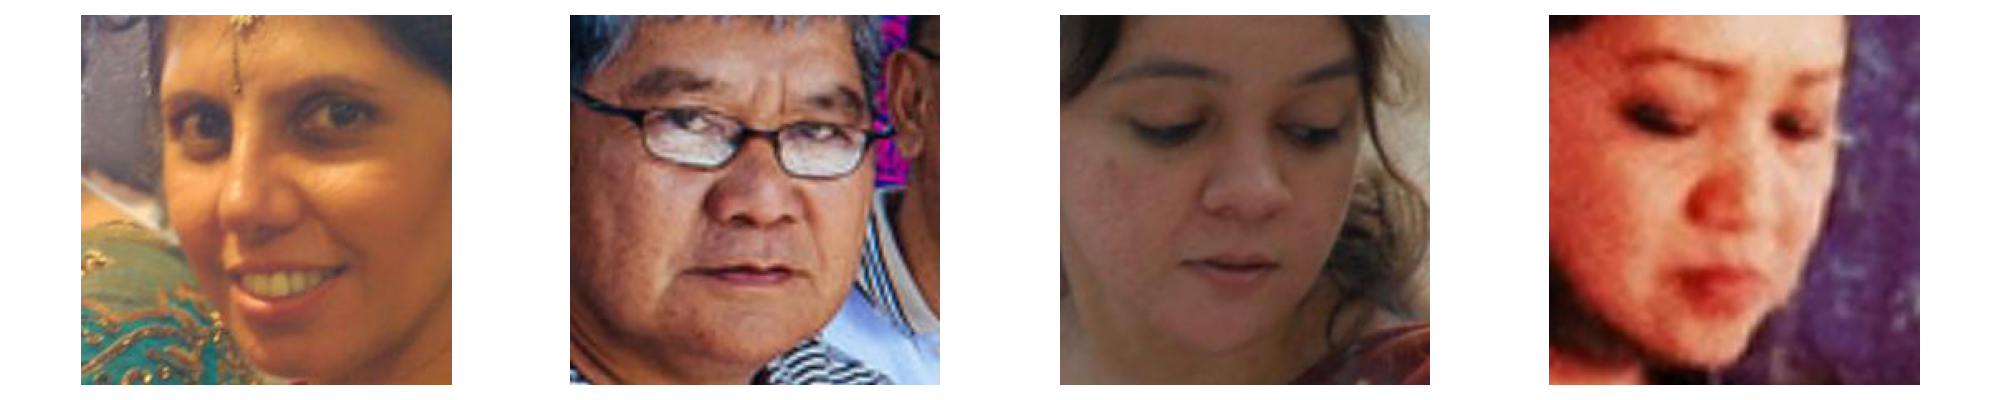
\includegraphics[width=1.1\textwidth]{ex_normal_dataset.png}
    \caption{一般人データセットの画像例}
    \label{fig:normal_ex}
\end{figure}
%======================



\section{実験結果}
\label{label:実験結果}
\subsection{Custom Modelの実験結果}
FairFaceが提供する学習済みモデルを本研究のタスクに合わせてカスタマイズしたResNet34を用いた実行結果を表\ref{tab:Custom}に示す。

\begin{table}[H]
\centering
\caption{Custom Model}
\label{tab:Custom}
\begin{tabular}{lrr}
\hline
 Epoch &  Train Accuracy &  Validation Accuracy \\
\hline
     1 &           99.48 &               100.00 \\
     2 &          100.00 &                99.99 \\
     3 &          100.00 &                99.99 \\
     4 &           99.97 &               100.00 \\
     5 &          100.00 &               100.00 \\
     6 &          100.00 &               100.00 \\
     7 &          100.00 &               100.00 \\
     8 &          100.00 &               100.00 \\
     9 &          100.00 &               100.00 \\
    10 &          100.00 &               100.00 \\
\hline
\end{tabular}
\end{table}
% 原因:過学習(valで結果が出ているから問題ない。)・データのリーク(=> 原因としてわかんない)・追加学習だからわかんないよ。
% 

考察:
学習済みモデルであるFairFaceに追加学習を施したCustom Modelは,エポック1からtrainの精度99.48\%,valの精度100.00\%と極めて高い精度を示した。エポック2以降もtrain,valの精度はほぼ100\%に達しており,この高精度が過学習によるものなのか,あるいは学習済みモデルや追加学習が原因となったものなのか,そもそも本モデルが画像のどの部分に着目して学習を行ったのかについても明確ではなく,高精度の要因の切り分けは困難である。さらに学習済みモデルについてGitHubや論文を参照しても詳細な情報は記載されておらず,内部の動作はブラックボックス化しており,原因の特定は困難である。\par

\subsection{Custom Modelの結果の透明性確保(仮説立て)}
\label{label:仮設立て}

前章で述べた過学習の可能性については,表\ref{tab:Custom}に示す結果から典型的な過学習の兆候は観察されず,過学習が生じているとは考えにくい。\par

以下に箇条書き形式で,なぜ表\ref{tab:Custom}のような高精度が実現できている原因について分析を行う。

\begin{itemize}
  \item \textbf{要因1. FairFaceの学習済みモデルが持つ広い表現能力}:  \\
  FairFace の学習済みモデルが持つ広い表現能力(性別・人種・年齢分類)に対し,本タスク(美男美女/一般人分類)が比較的容易な問題であったため,追加学習によって早期に分離境界を発見でき,このような高精度になったと考えられる。

  \item \textbf{要因2. パラメータ調整の違い}:  \\
  FairFaceモデルが高精度を示した背景には,適切なパラメータ調整が行われていた可能性がある.(しかしながら,文献\cite{karkkainenFairFace}やGitHub上に公開されているのは予測用のコードのみであり,具体的な調整手法やその根拠については明記されていない.)

  \item \textbf{要因3. 構築したデータセットに起因する要素}:
  \begin{itemize}
    \item FairFaceでは文献\cite{karkkainenFairFace}において約108,501枚の学習用画像が使用されている一方,本研究で用いたデータセットは,trainで約31,000枚,testで約7,800枚と画像数に大きな差がある.この画像数の違いが,学習モデルに影響を及ぼしている可能性がある.
    \item 一般人のデータについては新たに収集せず,FairFaceの学習済みモデルで既に使用された画像からダウンサンプリングして再利用している.そのため,モデルが顔以外の背景情報に依存して分類を行う傾向が生じた可能性がある.
  \end{itemize}
\end{itemize}
% we constructed a novel face image dataset containing 108,501 images which is balanced on Race.  

追加学習を行って100\%の精度を達成したが,この精度の妥当性を検証する。
上記仮説に基づき,違うアプローチとして,新規に学習を行い,それらと追加学習を行ったものを比較し,精度や追加学習を行ったため元のFairFaceの性別・人種・年齢分類と比べて美男美女・一般人の二値分類タスクが簡単だったのかを確かめる。
ここで,新規学習で用意したモデルはResNet18,ResNet34,ResNet50とEfficientNet\_b0であり,これらはCustom Modelと同じパラメータ調整を行った。


\section{仮説検証1:新規学習}
ResNet18,ResNet34,ResNet50とEfficientNetのモデルで新規学習を行なった実行結果を表\ref{tab:ResNet18},表\ref{tab:ResNet34},表\ref{tab:ResNet50},表\ref{tab:efficientnet}に示す。

\subsection{ResNet 18}
\begin{table}[H]
\centering
\caption{ResNet-18}
\label{tab:ResNet18}
\begin{tabular}{lrr}
\hline
 Epoch &  Train Accuracy &  Validation Accuracy \\
\hline
     1 &           97.92 &                99.28 \\
     2 &           99.23 &                99.22 \\
     3 &           99.47 &                99.53 \\
     4 &           99.61 &                99.48 \\
     5 &           99.68 &                99.52 \\
     6 &           99.76 &                99.38 \\
     7 &           99.83 &                99.59 \\
     8 &           99.83 &                99.51 \\
     9 &           99.88 &                99.45 \\
    10 &           99.88 &                99.52 \\
\hline
\end{tabular}
\end{table}



\subsubsection*{ResNet 18の考察:}
ResNet-18は,Train Accuracyの精度が97.92\%から99.88\%まで順調に向上した一方,Validation Accuracyの精度は99.2\%から99.6\%の範囲で安定して推移していることがわかる。Train AccuracyとValidation Accuracyの値が激しく乖離しておらず,適切に学習できていることが示唆される。またエポック3以降は,学習精度と検証精度がほぼ同程度の水準で推移しており,安定した汎化性能を有していると評価できる。


\subsection{ResNet 34}
\begin{table}[h]
\centering
\caption{ResNet-34}
\label{tab:ResNet34}
\begin{tabular}{lrr}
\hline
 Epoch &  Train Accuracy &  Validation Accuracy \\
\hline
     1 &           97.74 &                99.08 \\
     2 &           99.27 &                99.34 \\
     3 &           99.40 &                99.27 \\
     4 &           99.55 &                99.50 \\
     5 &           99.59 &                99.40 \\
     6 &           99.65 &                99.27 \\
     7 &           99.72 &                99.31 \\
     8 &           99.80 &                99.49 \\
     9 &           99.79 &                99.56 \\
    10 &           99.84 &                99.47 \\
\hline
\end{tabular}
\end{table}

\subsubsection*{ResNet 34の考察:}
ResNet-34の結果は,ResNet-18と同様の傾向を示している。エポック10において,Train Accuracyが99.84,Validation Accuracyが99.47に達しており,ResNet18よりも若干低い性能を示している。前述のResNet18よりも層が深くなっているものの,検証の精度自体に著しい向上が見られなかったことから,ResNet18の時点で十分にモデルの表現能力が達成されており,これ以上層を増やしてもこれ以上の性能向上は見込めないだろう。

\subsection{ResNet 50}

\begin{table}[H]
\centering
\caption{ResNet-50}
\label{tab:ResNet50}
\begin{tabular}{lrr}
\hline
 Epoch &  Train Accuracy &  Validation Accuracy \\
\hline
     1 &           95.26 &                98.58 \\
     2 &           98.69 &                98.76 \\
     3 &           99.10 &                99.20 \\
     4 &           99.32 &                99.25 \\
     5 &           99.39 &                99.34 \\
     6 &           99.50 &                99.37 \\
     7 &           99.54 &                99.40 \\
     8 &           99.66 &                99.28 \\
     9 &           99.71 &                99.36 \\
    10 &           99.75 &                99.39 \\
\hline
\end{tabular}
\end{table}

\subsubsection*{ResNet 50の考察:}
ResNet-18やResNet-34の性能を上回ることはなく,ResNetでは層を$18,34,50 \cdots$と深くしても顕著な性能向上は見られなかった。さらには訓練初期のTrain Accuracyが他のResNetモデルより低い(95.26\%)ことから,モデルの複雑性が増した分学習の収束に時間を要する可能性が考えられる。本データセットの分類タスクの複雑性に対して,ResNet-18の時点ですでにモデルの表現力が十分であったことが考えられる。
%モデルの層を増やすよりかはパラメータ調整の方が有益であろう。


\subsection{EfficientNet\_b0}

\begin{table}[H]
\centering
\caption{EfficientNet}
\label{tab:efficientnet}
\begin{tabular}{lrr}
\hline
 Epoch &  Train Accuracy &  Validation Accuracy \\
\hline
     1 &           94.47 &                98.76 \\
     2 &           99.00 &                99.19 \\
     3 &           99.40 &                99.54 \\
     4 &           99.63 &                99.59 \\
     5 &           99.79 &                99.79 \\
     6 &           99.85 &                99.82 \\
     7 &           99.89 &                99.94 \\
     8 &           99.92 &                99.96 \\
     9 &           99.93 &                99.87 \\
    10 &           99.95 &                99.96 \\
\hline
\end{tabular}
\end{table}


\subsubsection*{EfficientNet\_b0の考察:}
エポック1の時点で既に高い精度を示しており,以降の学習過程においてもtrain,valの精度の両方がエポックの進行と共に安定して向上し,最終的にはエポック10で99.86という高い値を更新している。EfficientNet は本タスクにおいて極めて高い表現力を有しており,少数のエポックでも十分な収束が得られることがわかる。Train Accuracyと Validation Accuracy の推移は類似しており,両者間に大きな乖離は見られないことから,過学習の兆候も確認されない。

\clearpage

\subsection{Custom Modelと新規学習の比較}
図\ref{fig:model_outputs_sorted }にCustom Modelと新規学習の実行結果をグラフとして示す。
%=======================

\begin{figure}[H]
  \centering

  % --- 1段目 ---
  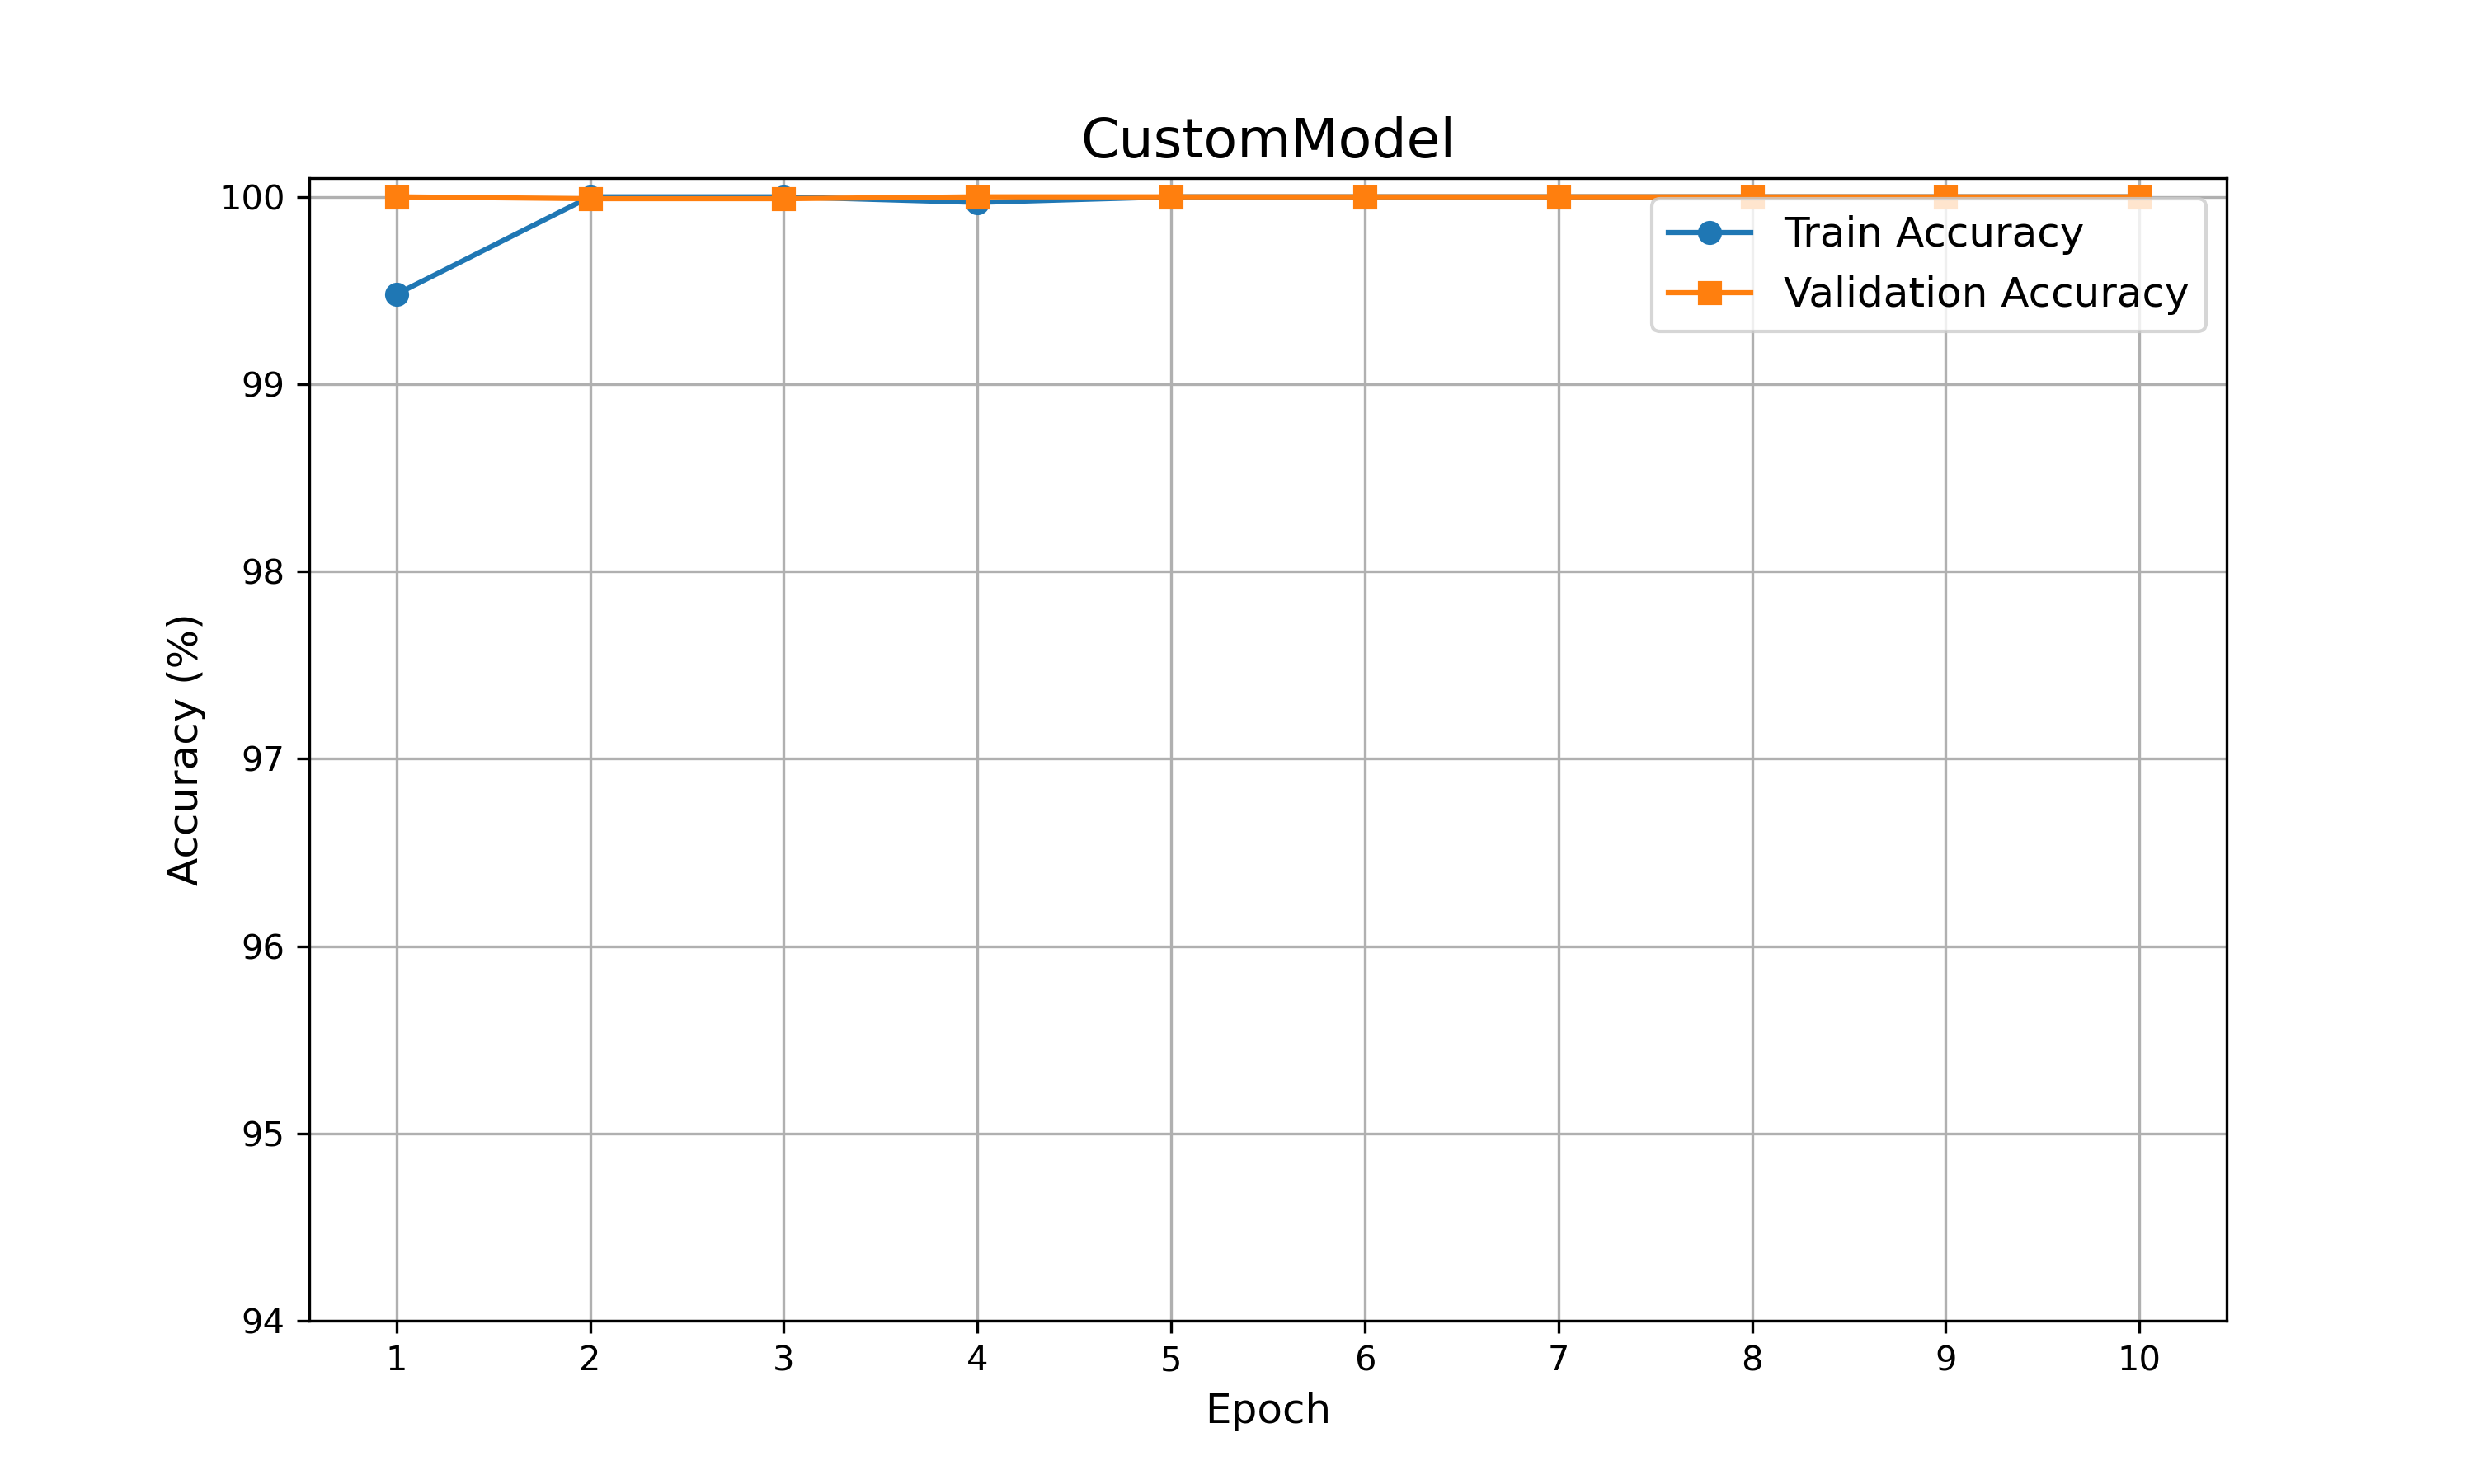
\includegraphics[width=0.48\textwidth]{CustomModel_output.png}
  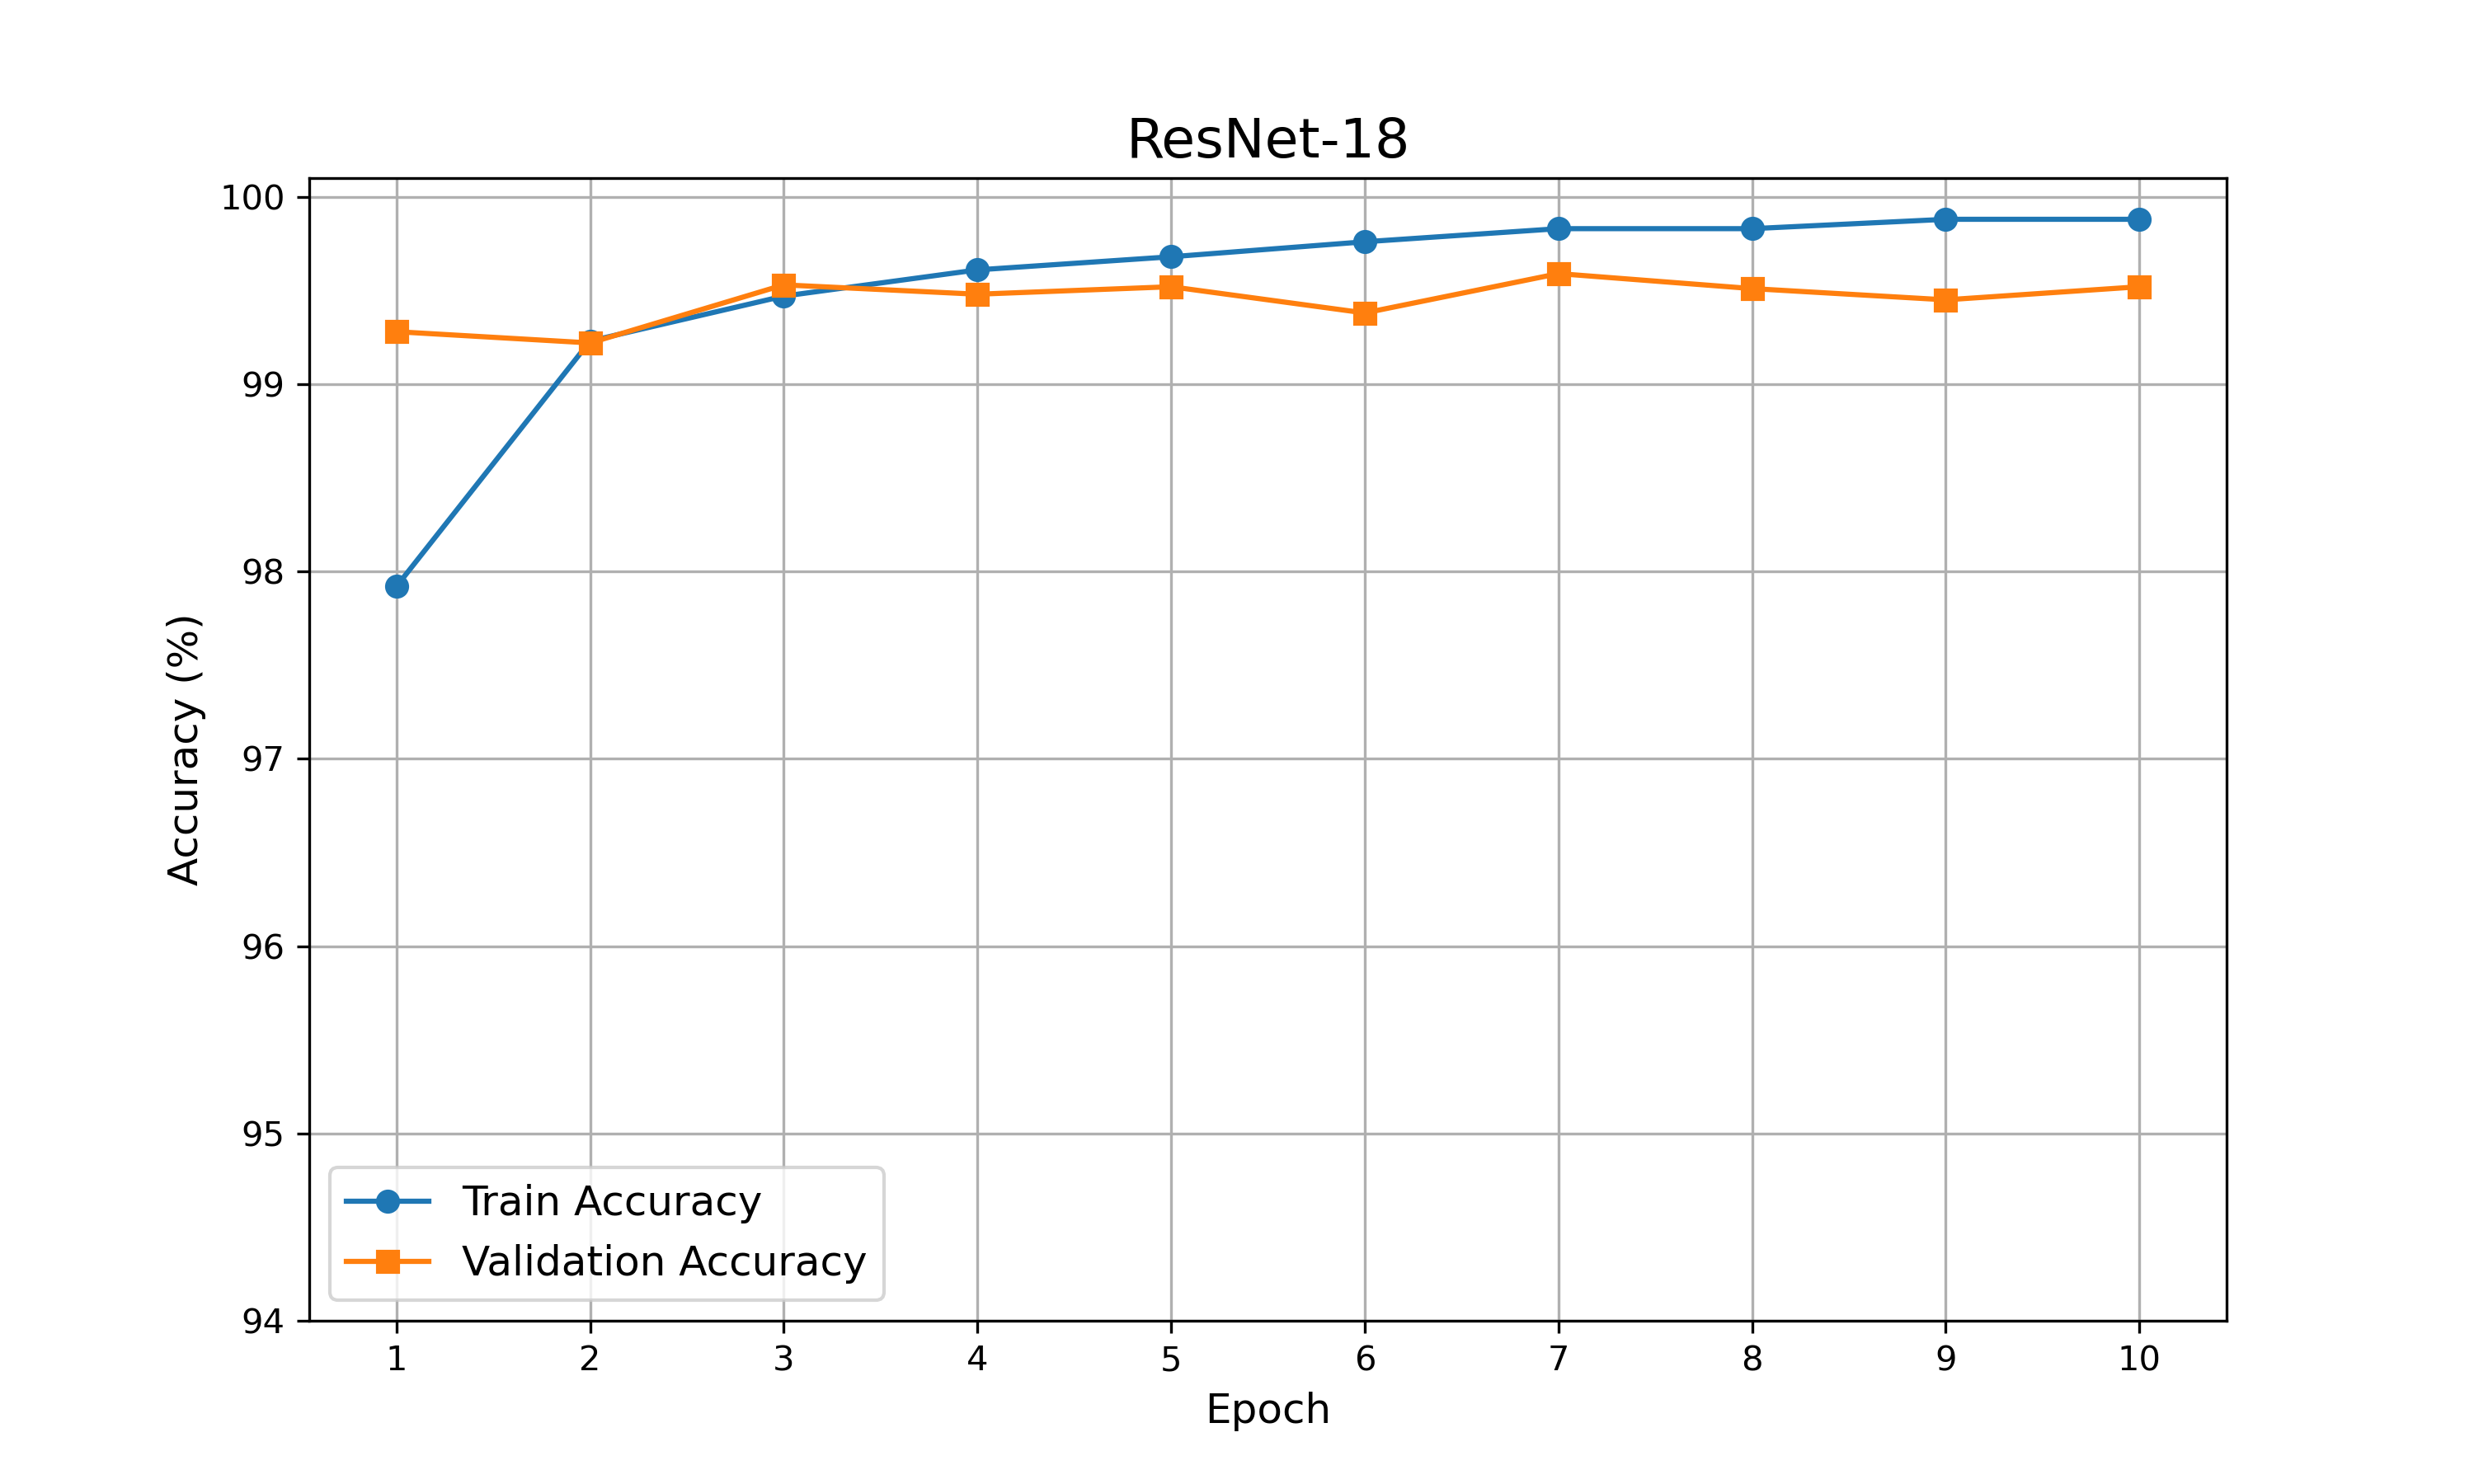
\includegraphics[width=0.48\textwidth]{ResNet-18_output.png}
  
  \vspace{0.3cm} % 縦間隔

  % --- 2段目 ---
  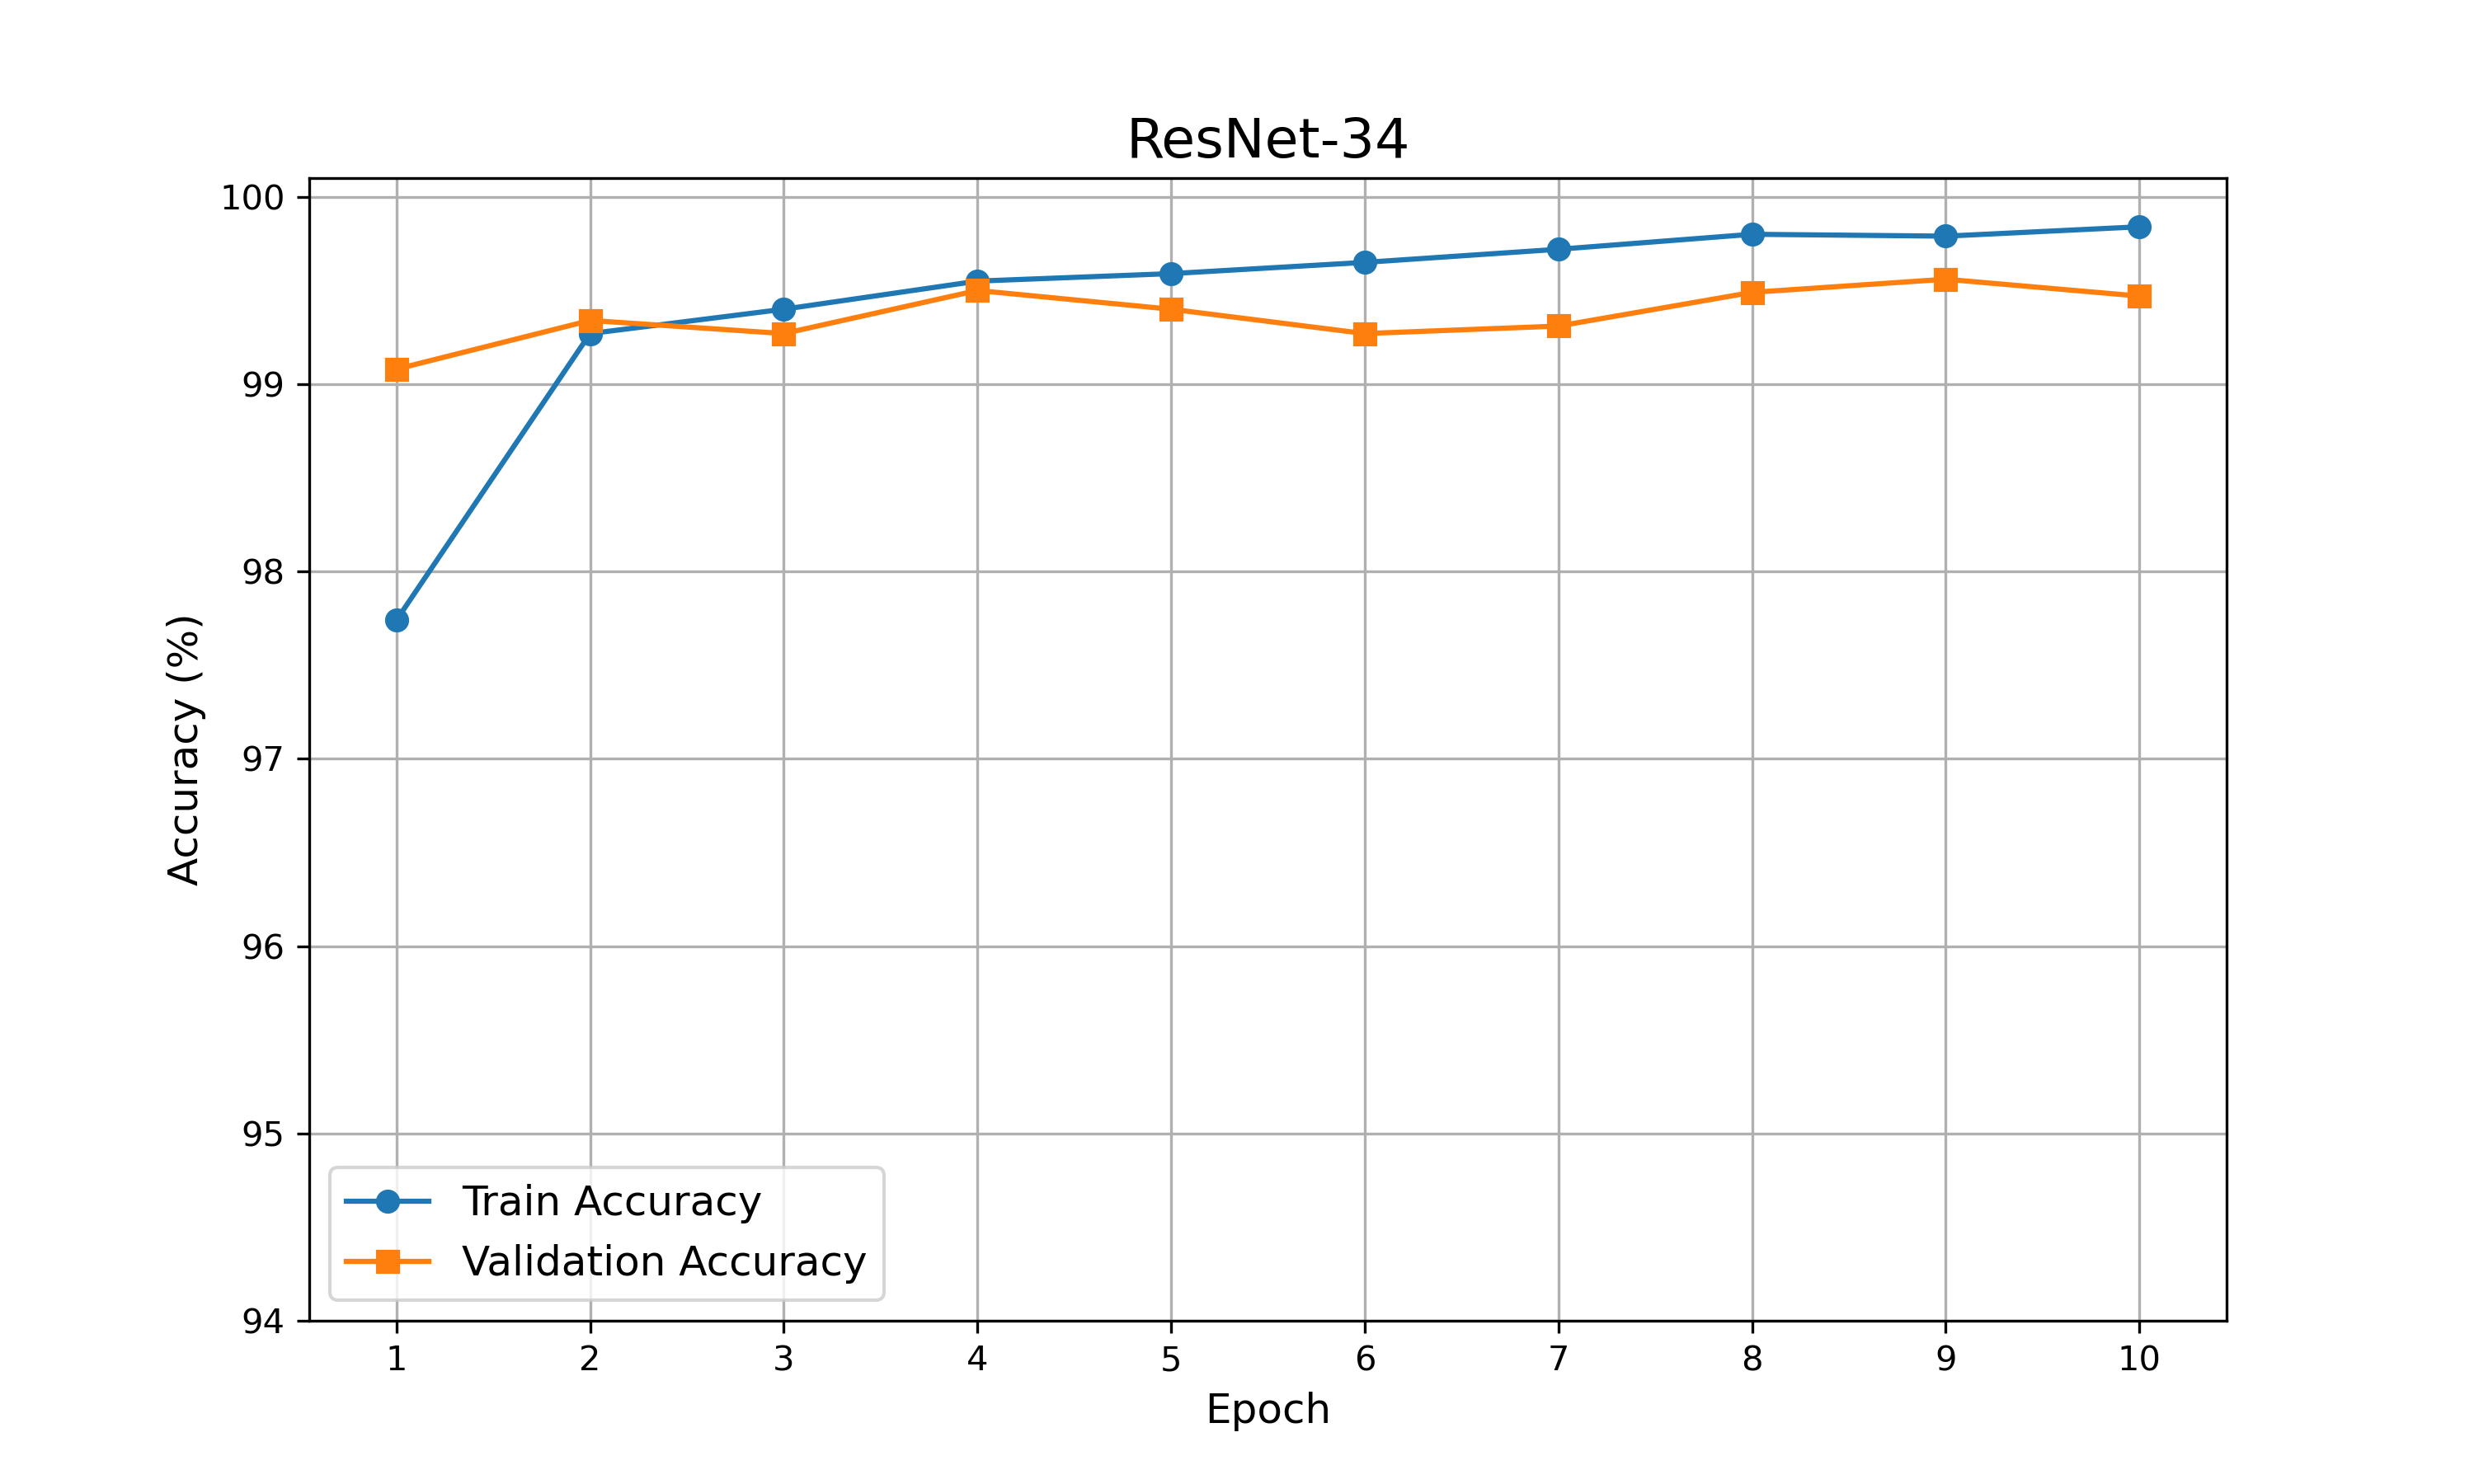
\includegraphics[width=0.48\textwidth]{ResNet-34_output.png}
  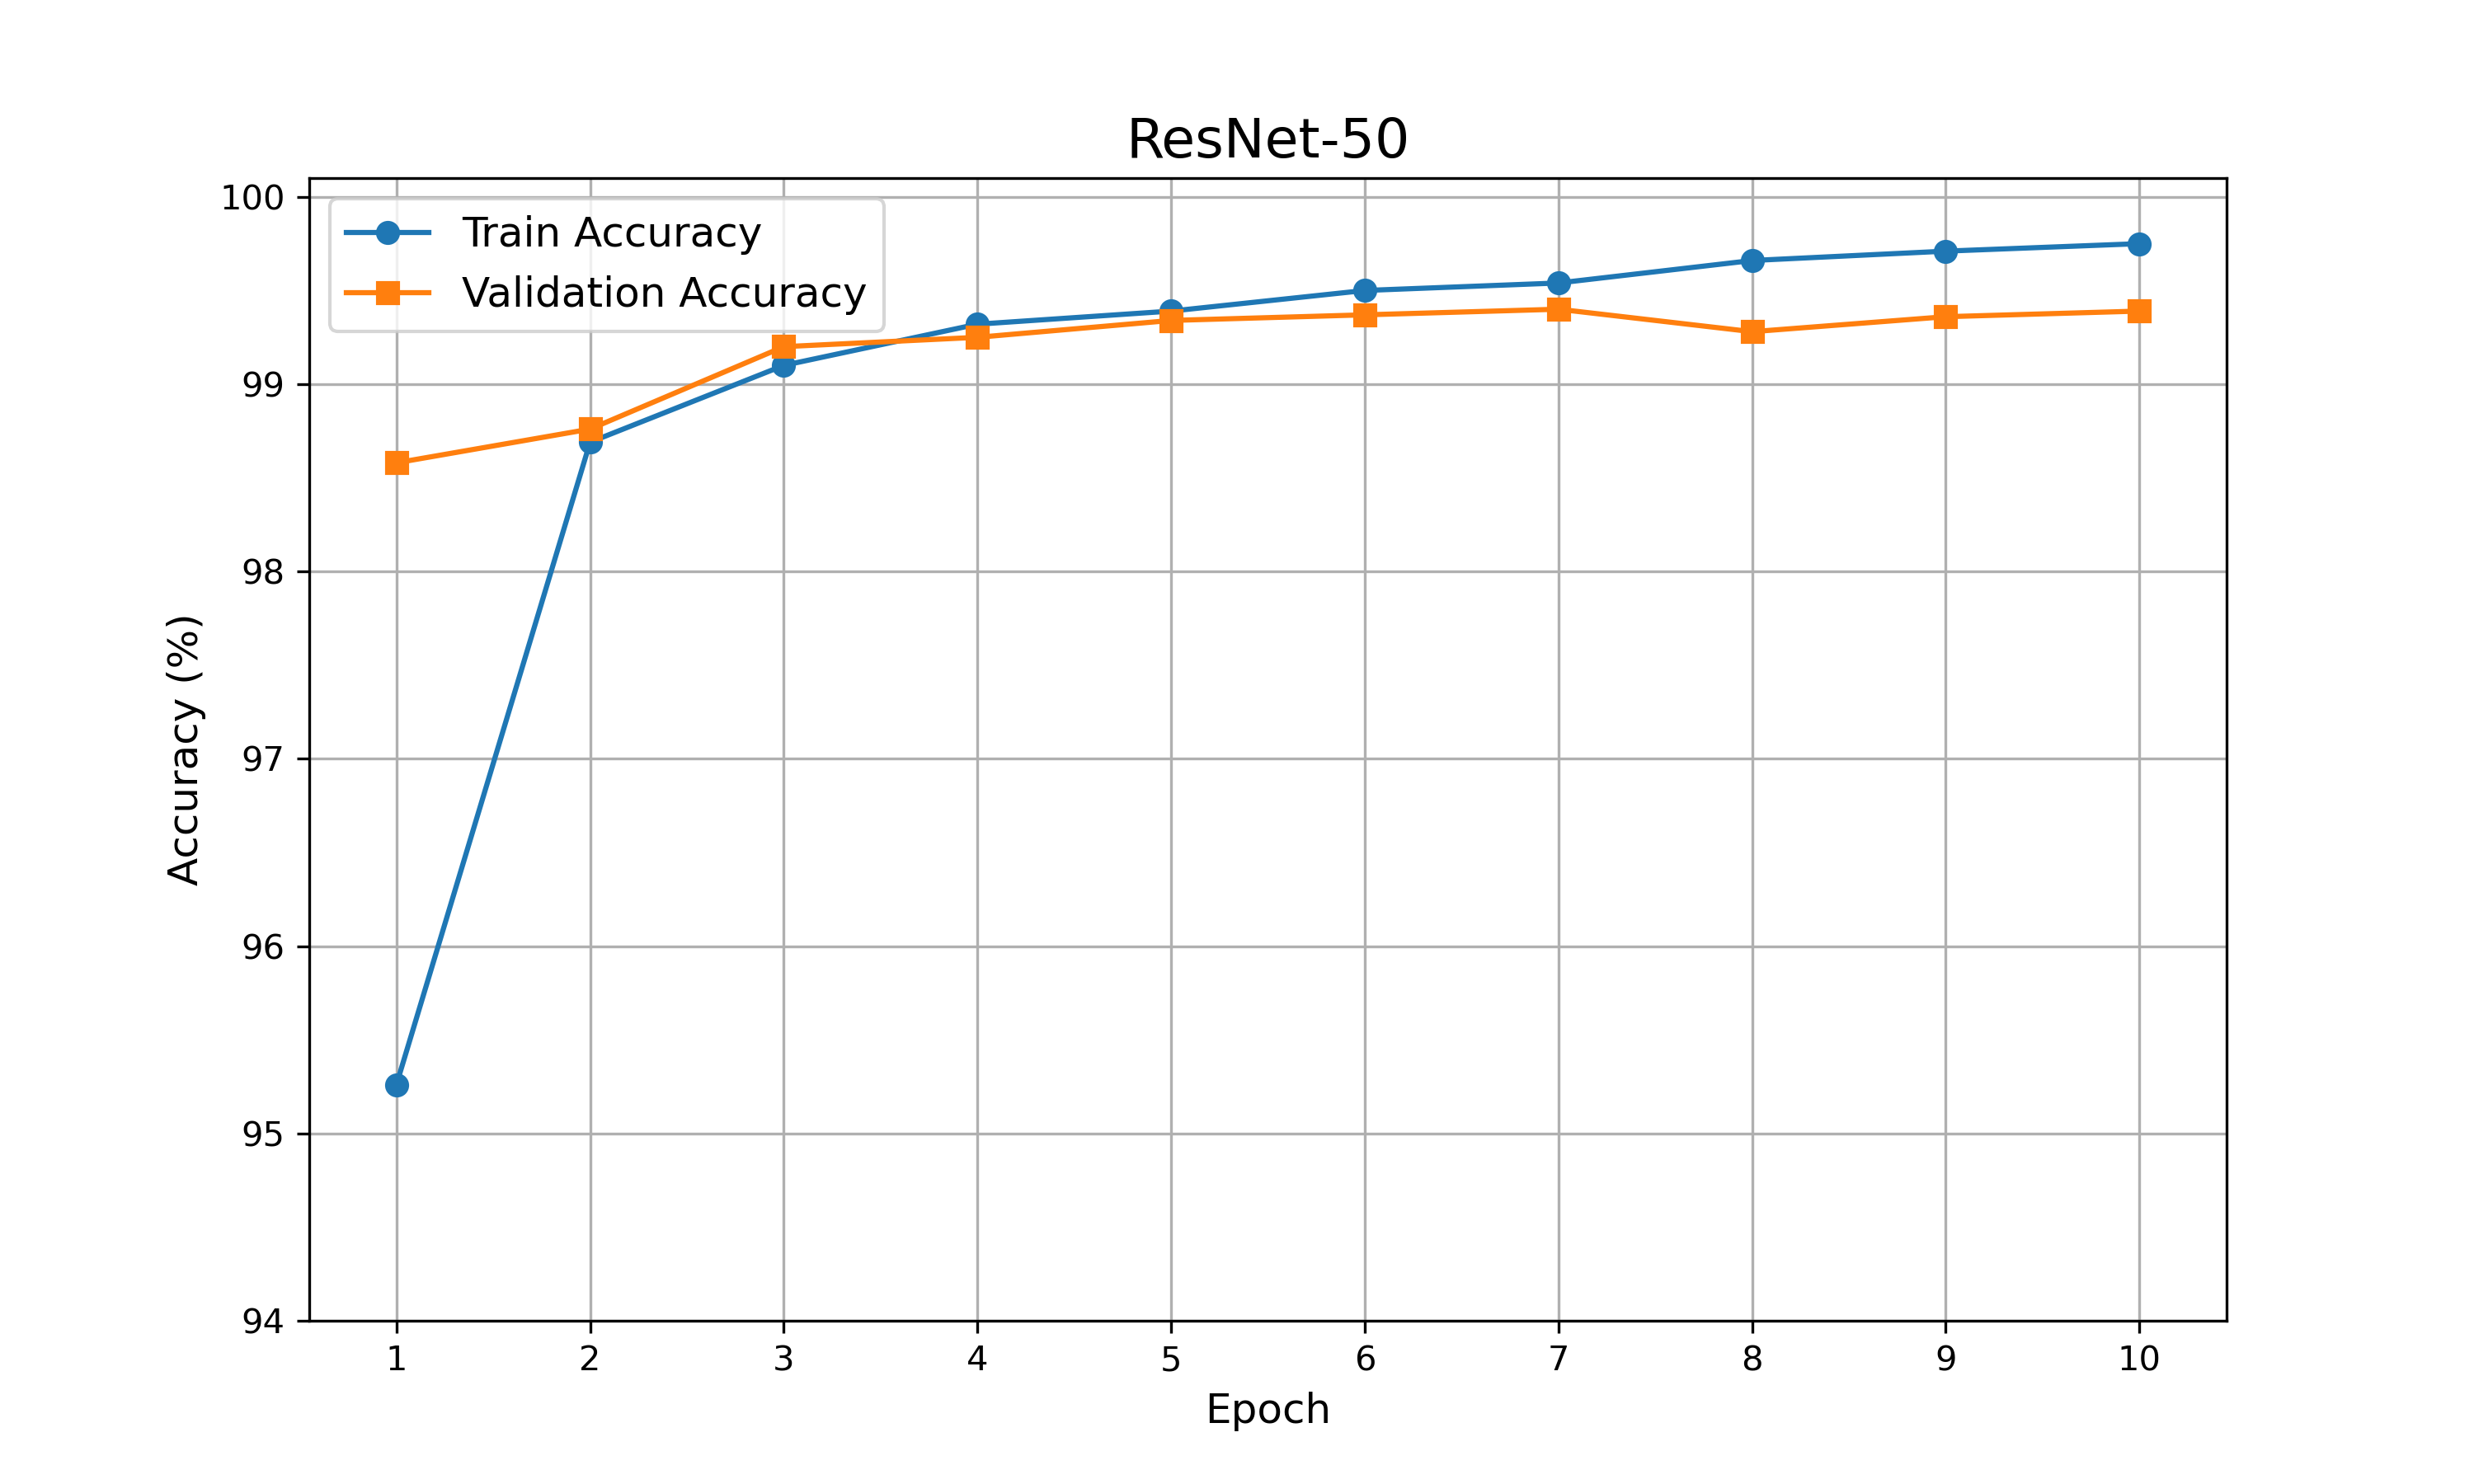
\includegraphics[width=0.48\textwidth]{ResNet-50_output.png}
  
  \vspace{0.3cm}

  % --- 3段目(中央寄せ) ---
  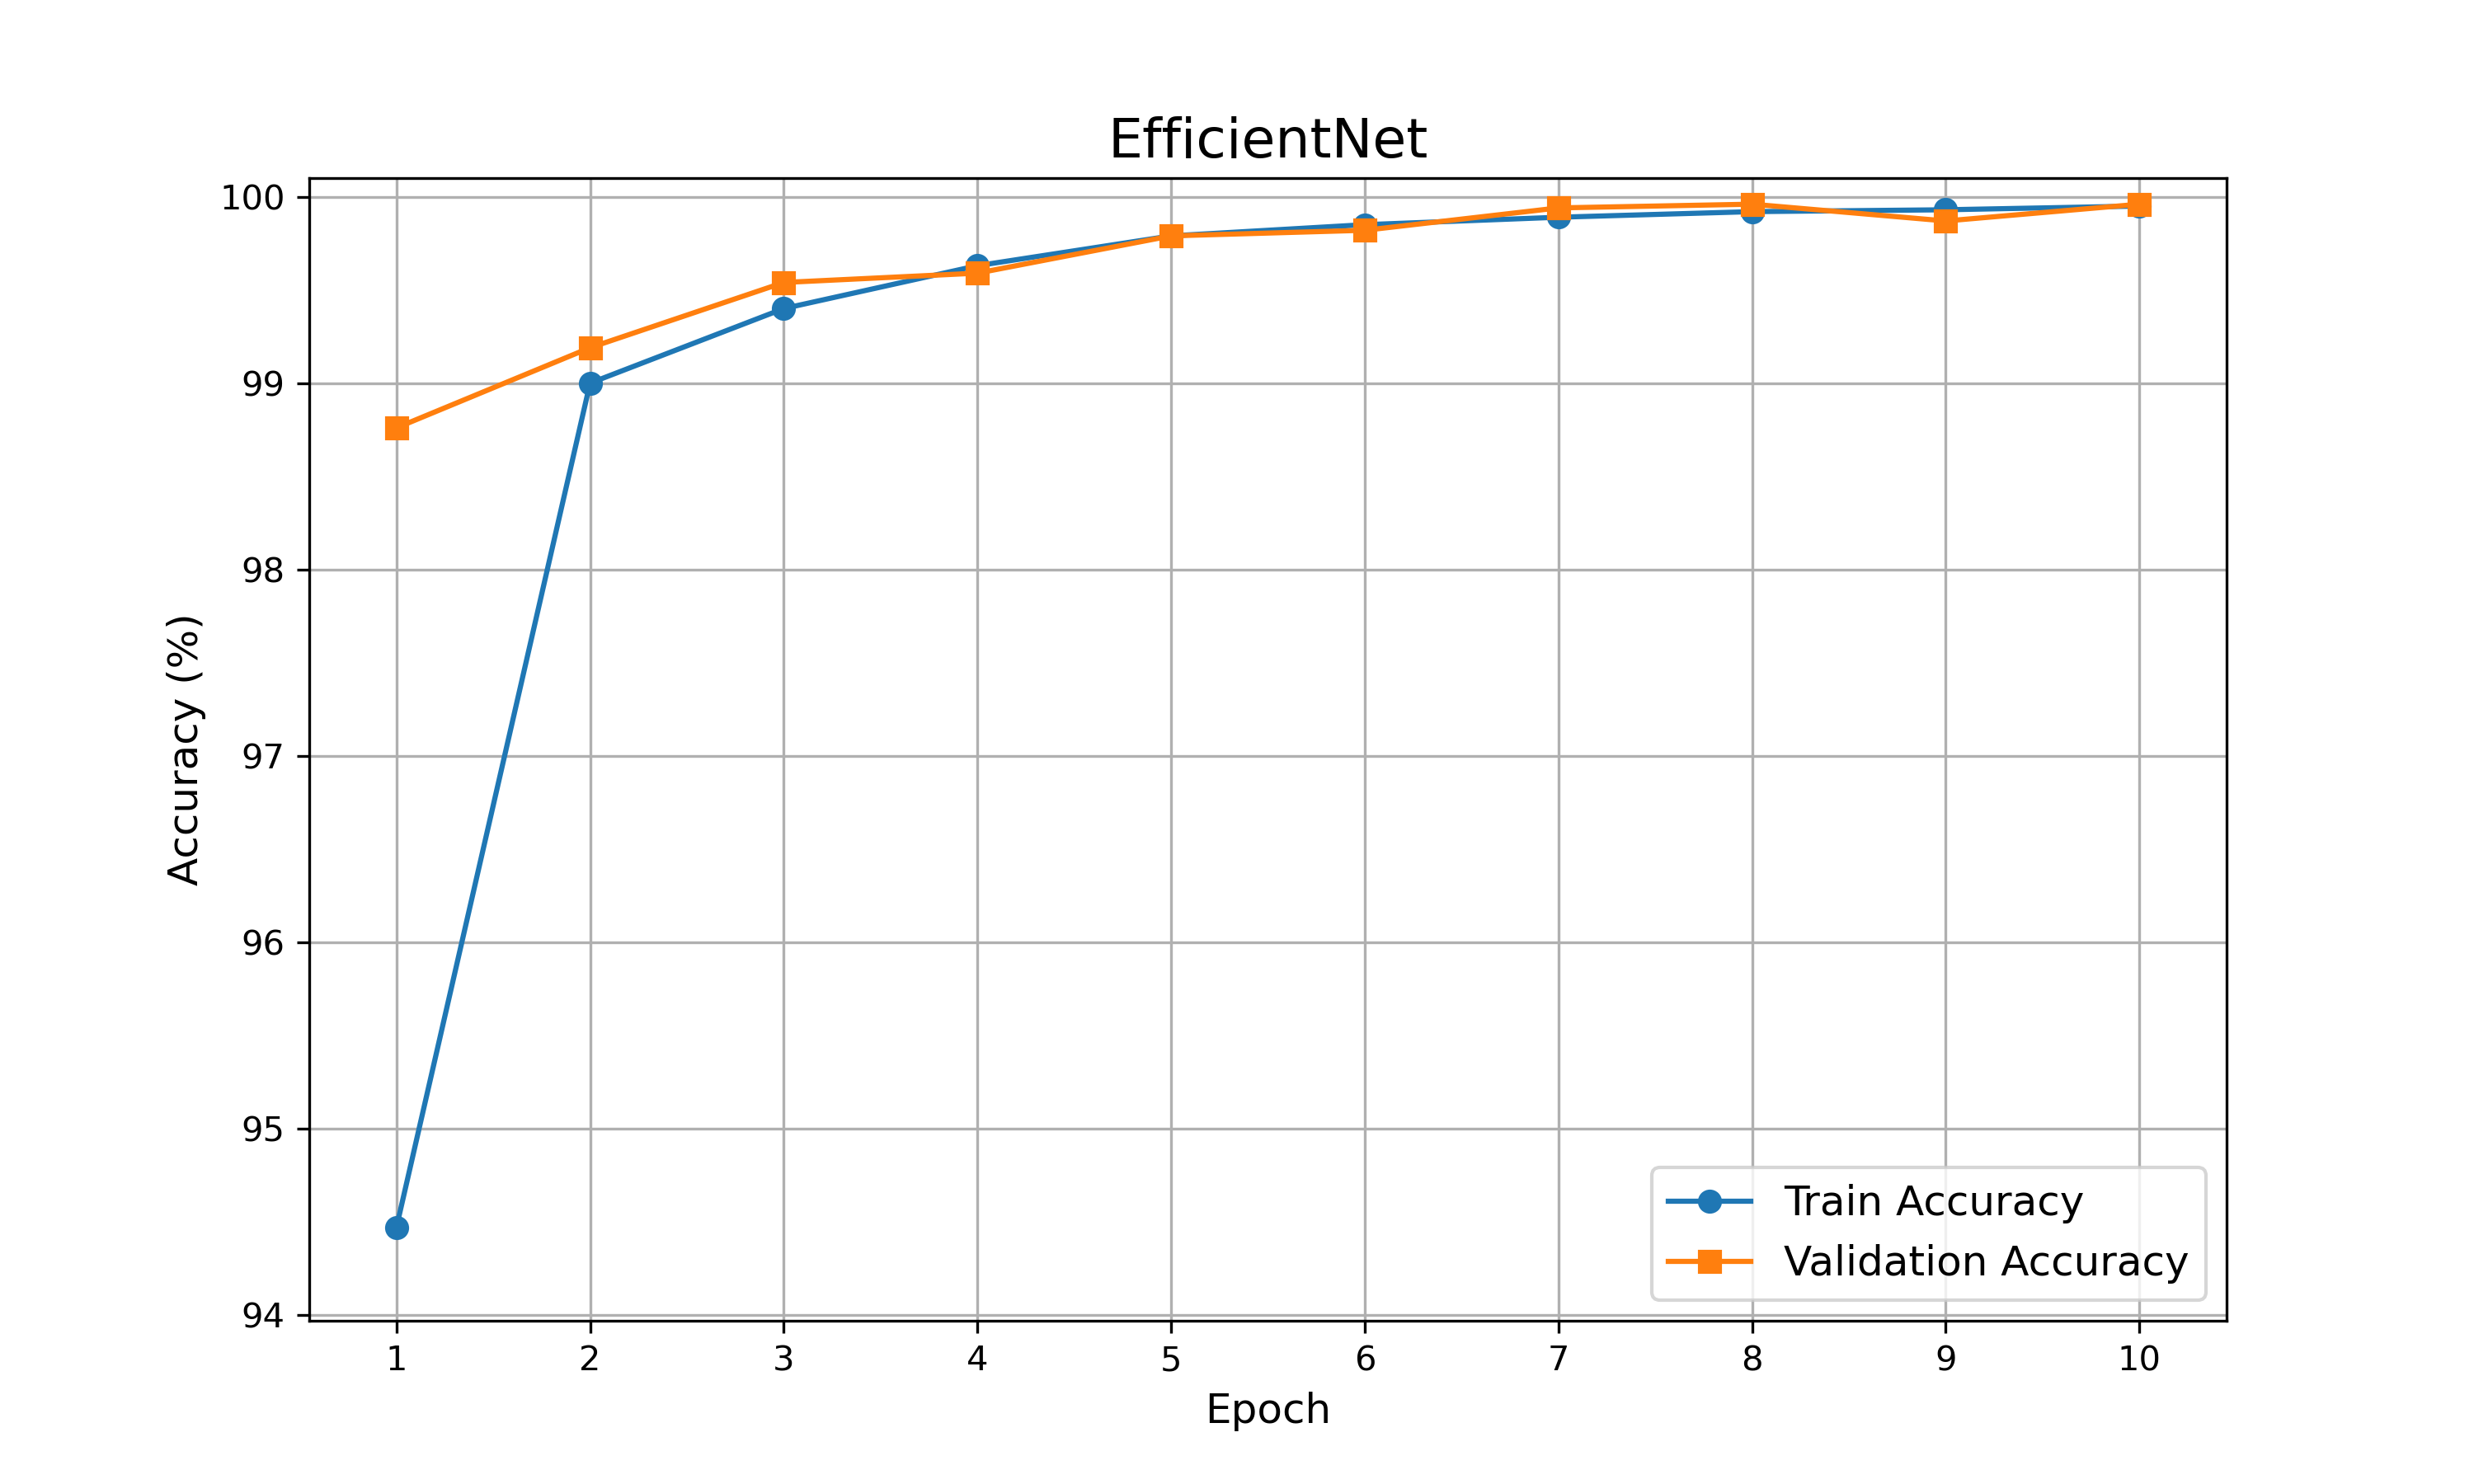
\includegraphics[width=0.6\textwidth]{EfficientNet_output.png}

  \caption{各モデルの出力結果(Custom Modelと新規学習モデル)}
  \label{fig:model_outputs_sorted}
\end{figure}

%=======================

Custom Modelがエポック1から高精度を実現できているものの,新規学習モデルについてもエポック1から95\%後半と高精度で実現できており,新規学習モデルはCustomModelと同様のパラメータ調整を行ったことからCustom Modelの高精度の原因がパラメータ調整によるものとは考えにくい。一方で新規学習したResNetやEfficientNetにとって美男美女・一般人の2値分類タスクがそもそも簡単なタスクであった可能性がある。そこで正しく顔のみを見て分類し,ここまで高い精度を実現できているかは不透明であるため,Grad-Camによる検証も行う。

%新規学習のモデルは,Custom Modelと比較しても高精度で実現できており,この新規学習のアプローチでは仮説の検証を行えなかった。


\clearpage

\section{仮説検証2:Grad-Camを用いたモデルの信頼性の検証}
\label{label:仮説検証2}
\subsection{検証の概要}
Grad-CAM(Gradient-weighted Class Activation Mapping)というCNNが画像のどの部分に注目して一般人か美男美女かの判断を下したのかをヒートマップとして可視化する技術がある。
図\ref{fig:gradcam_good},図\ref{fig:gradcam_normal}にGrad-CAMを用いてモデルごとに美男美女(good)と一般人(normal)の各データの平均したヒートマップを示す。
本研究で得られた99\%超という検証精度の原因を探る。
各画像は以下に示すモデルを適用した結果である。
\begin{itemize}
	\item 1行目
	\begin{itemize}
	\item 追加学習したモデル:Custom
	\item EfficientNet\_b0
	\item ResNet18
	\end{itemize}
	\item 2行目
	\begin{itemize}
	\item ResNet34
	\item ResNet50
	\end{itemize}
\end{itemize}


\subsection{検証結果}
%======================
\begin{figure}[H]
    \centering
    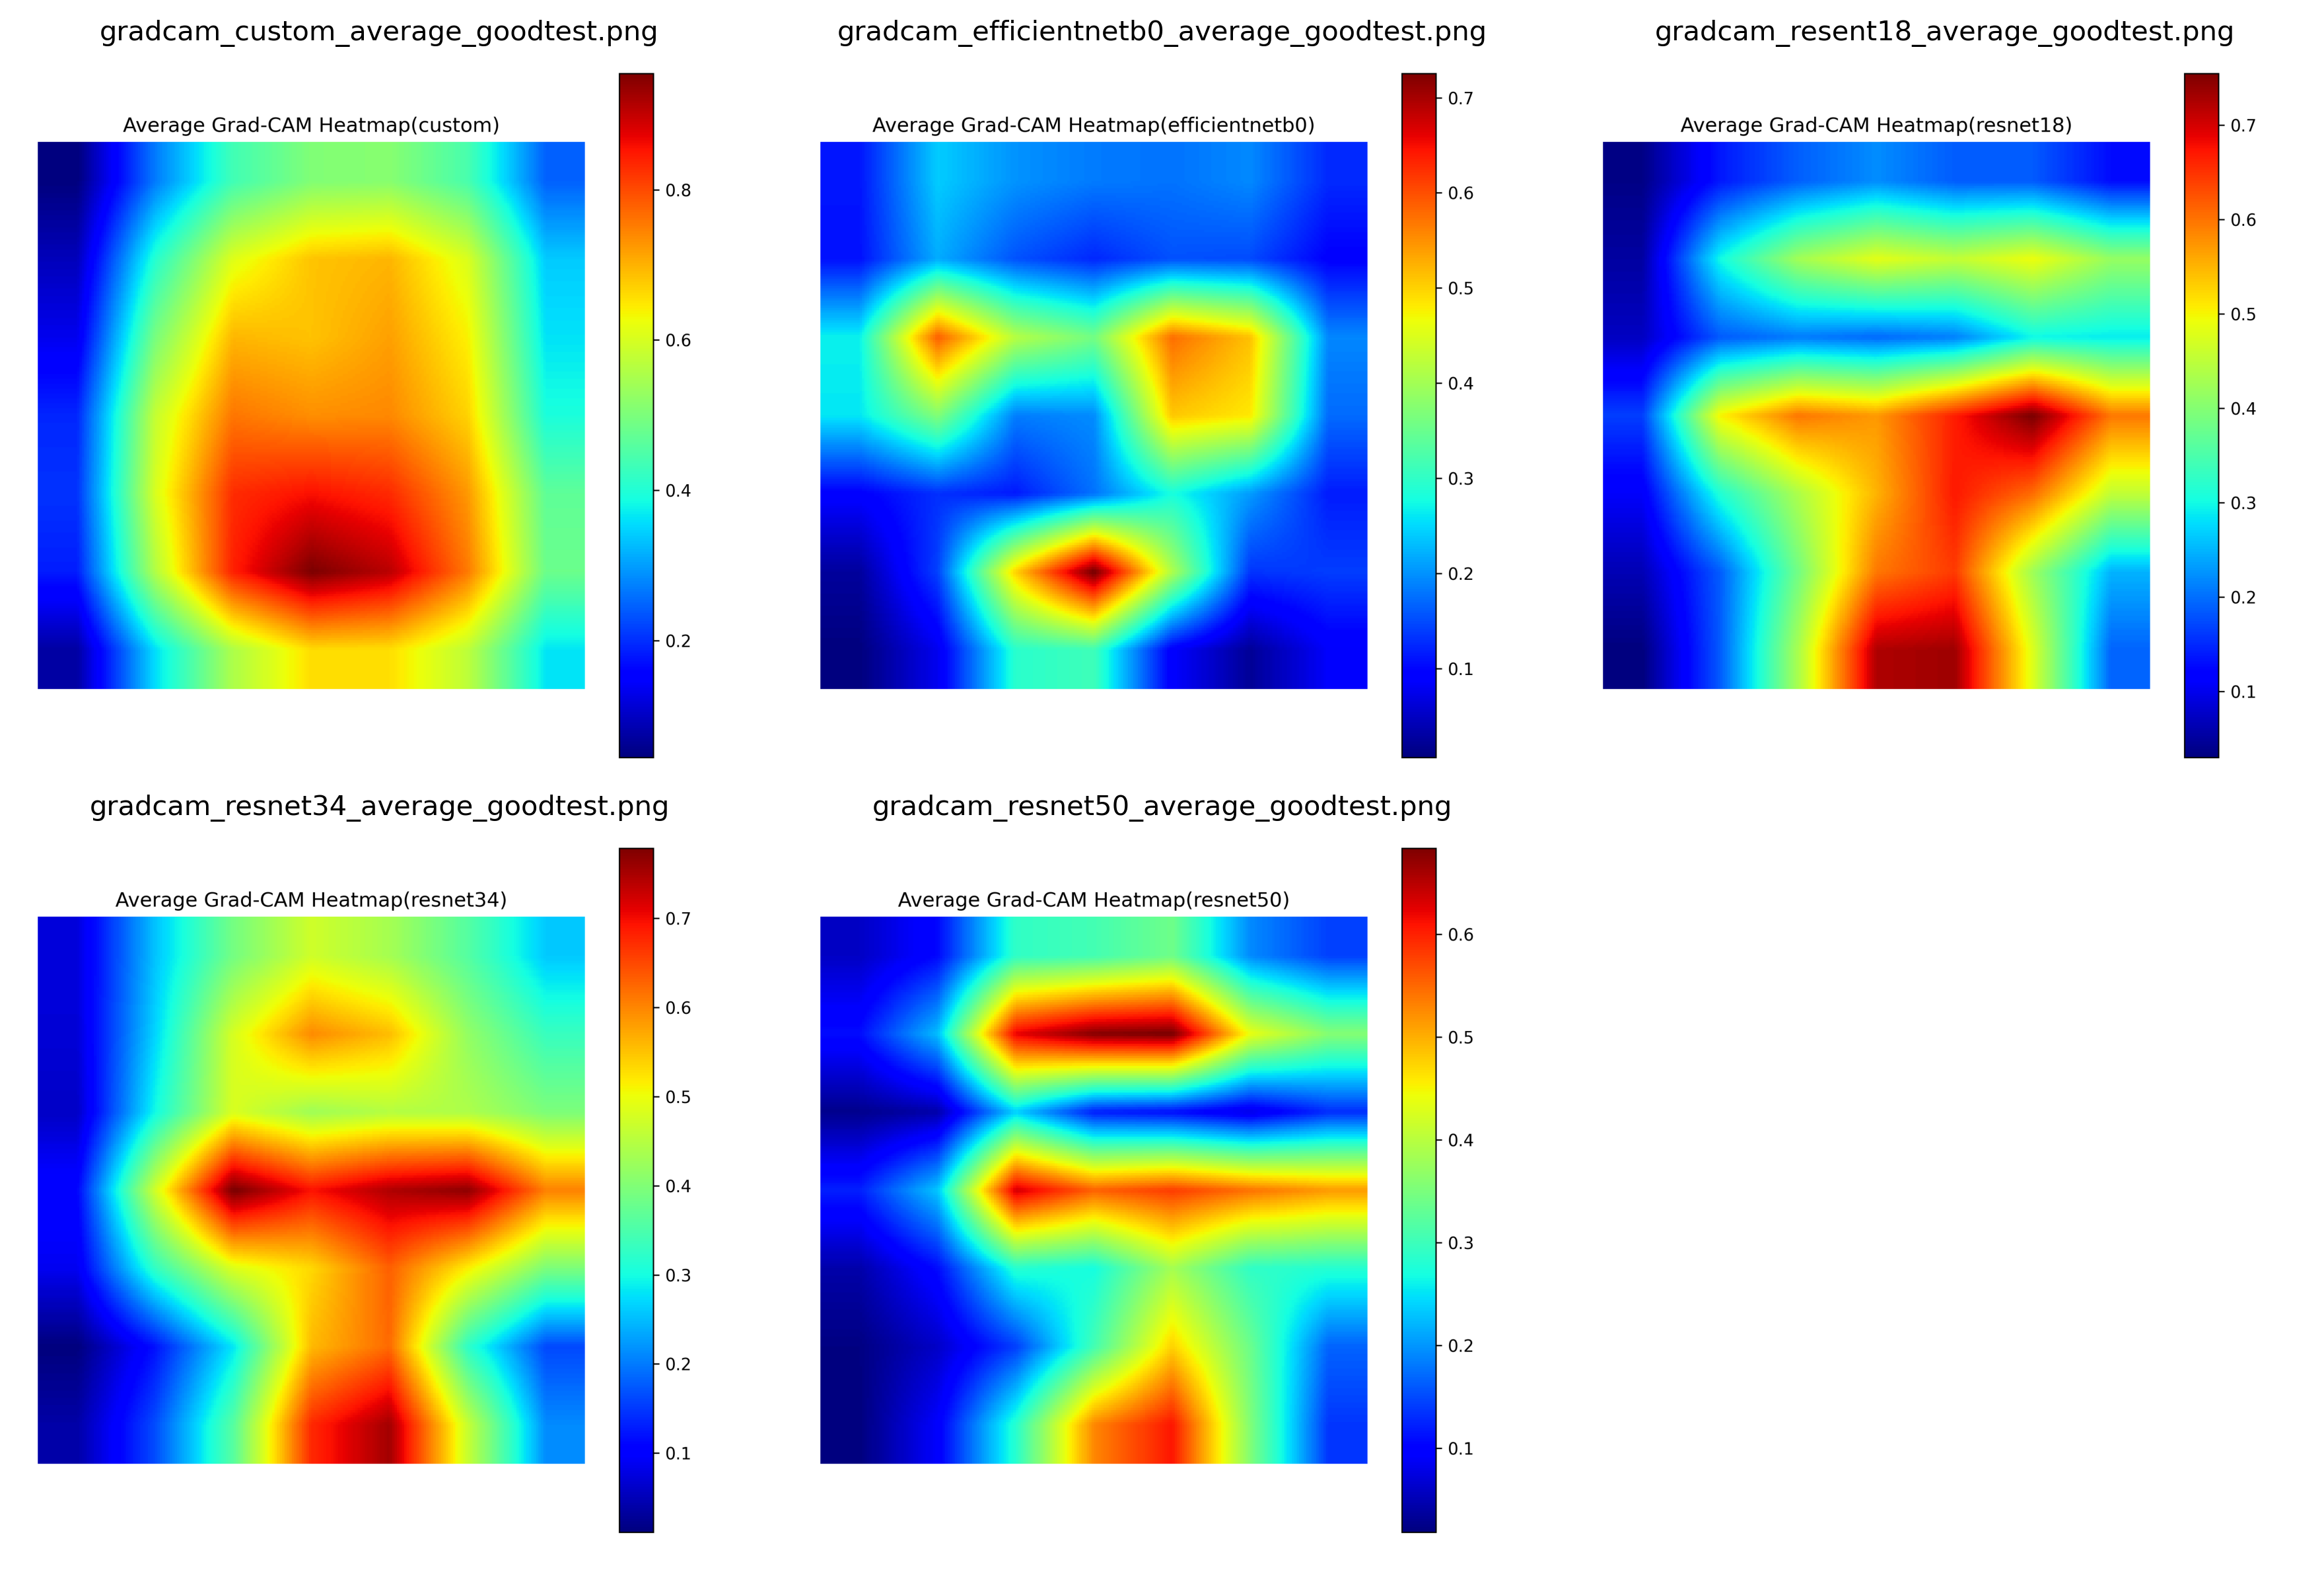
\includegraphics[width=1.1\textwidth]{combined_images_good.png}
    \caption{Grad-CAMを用いた美男美女の判断根拠の可視化}
    \label{fig:gradcam_good}
\end{figure}
%======================
%======================
\begin{figure}[H]
    \centering
    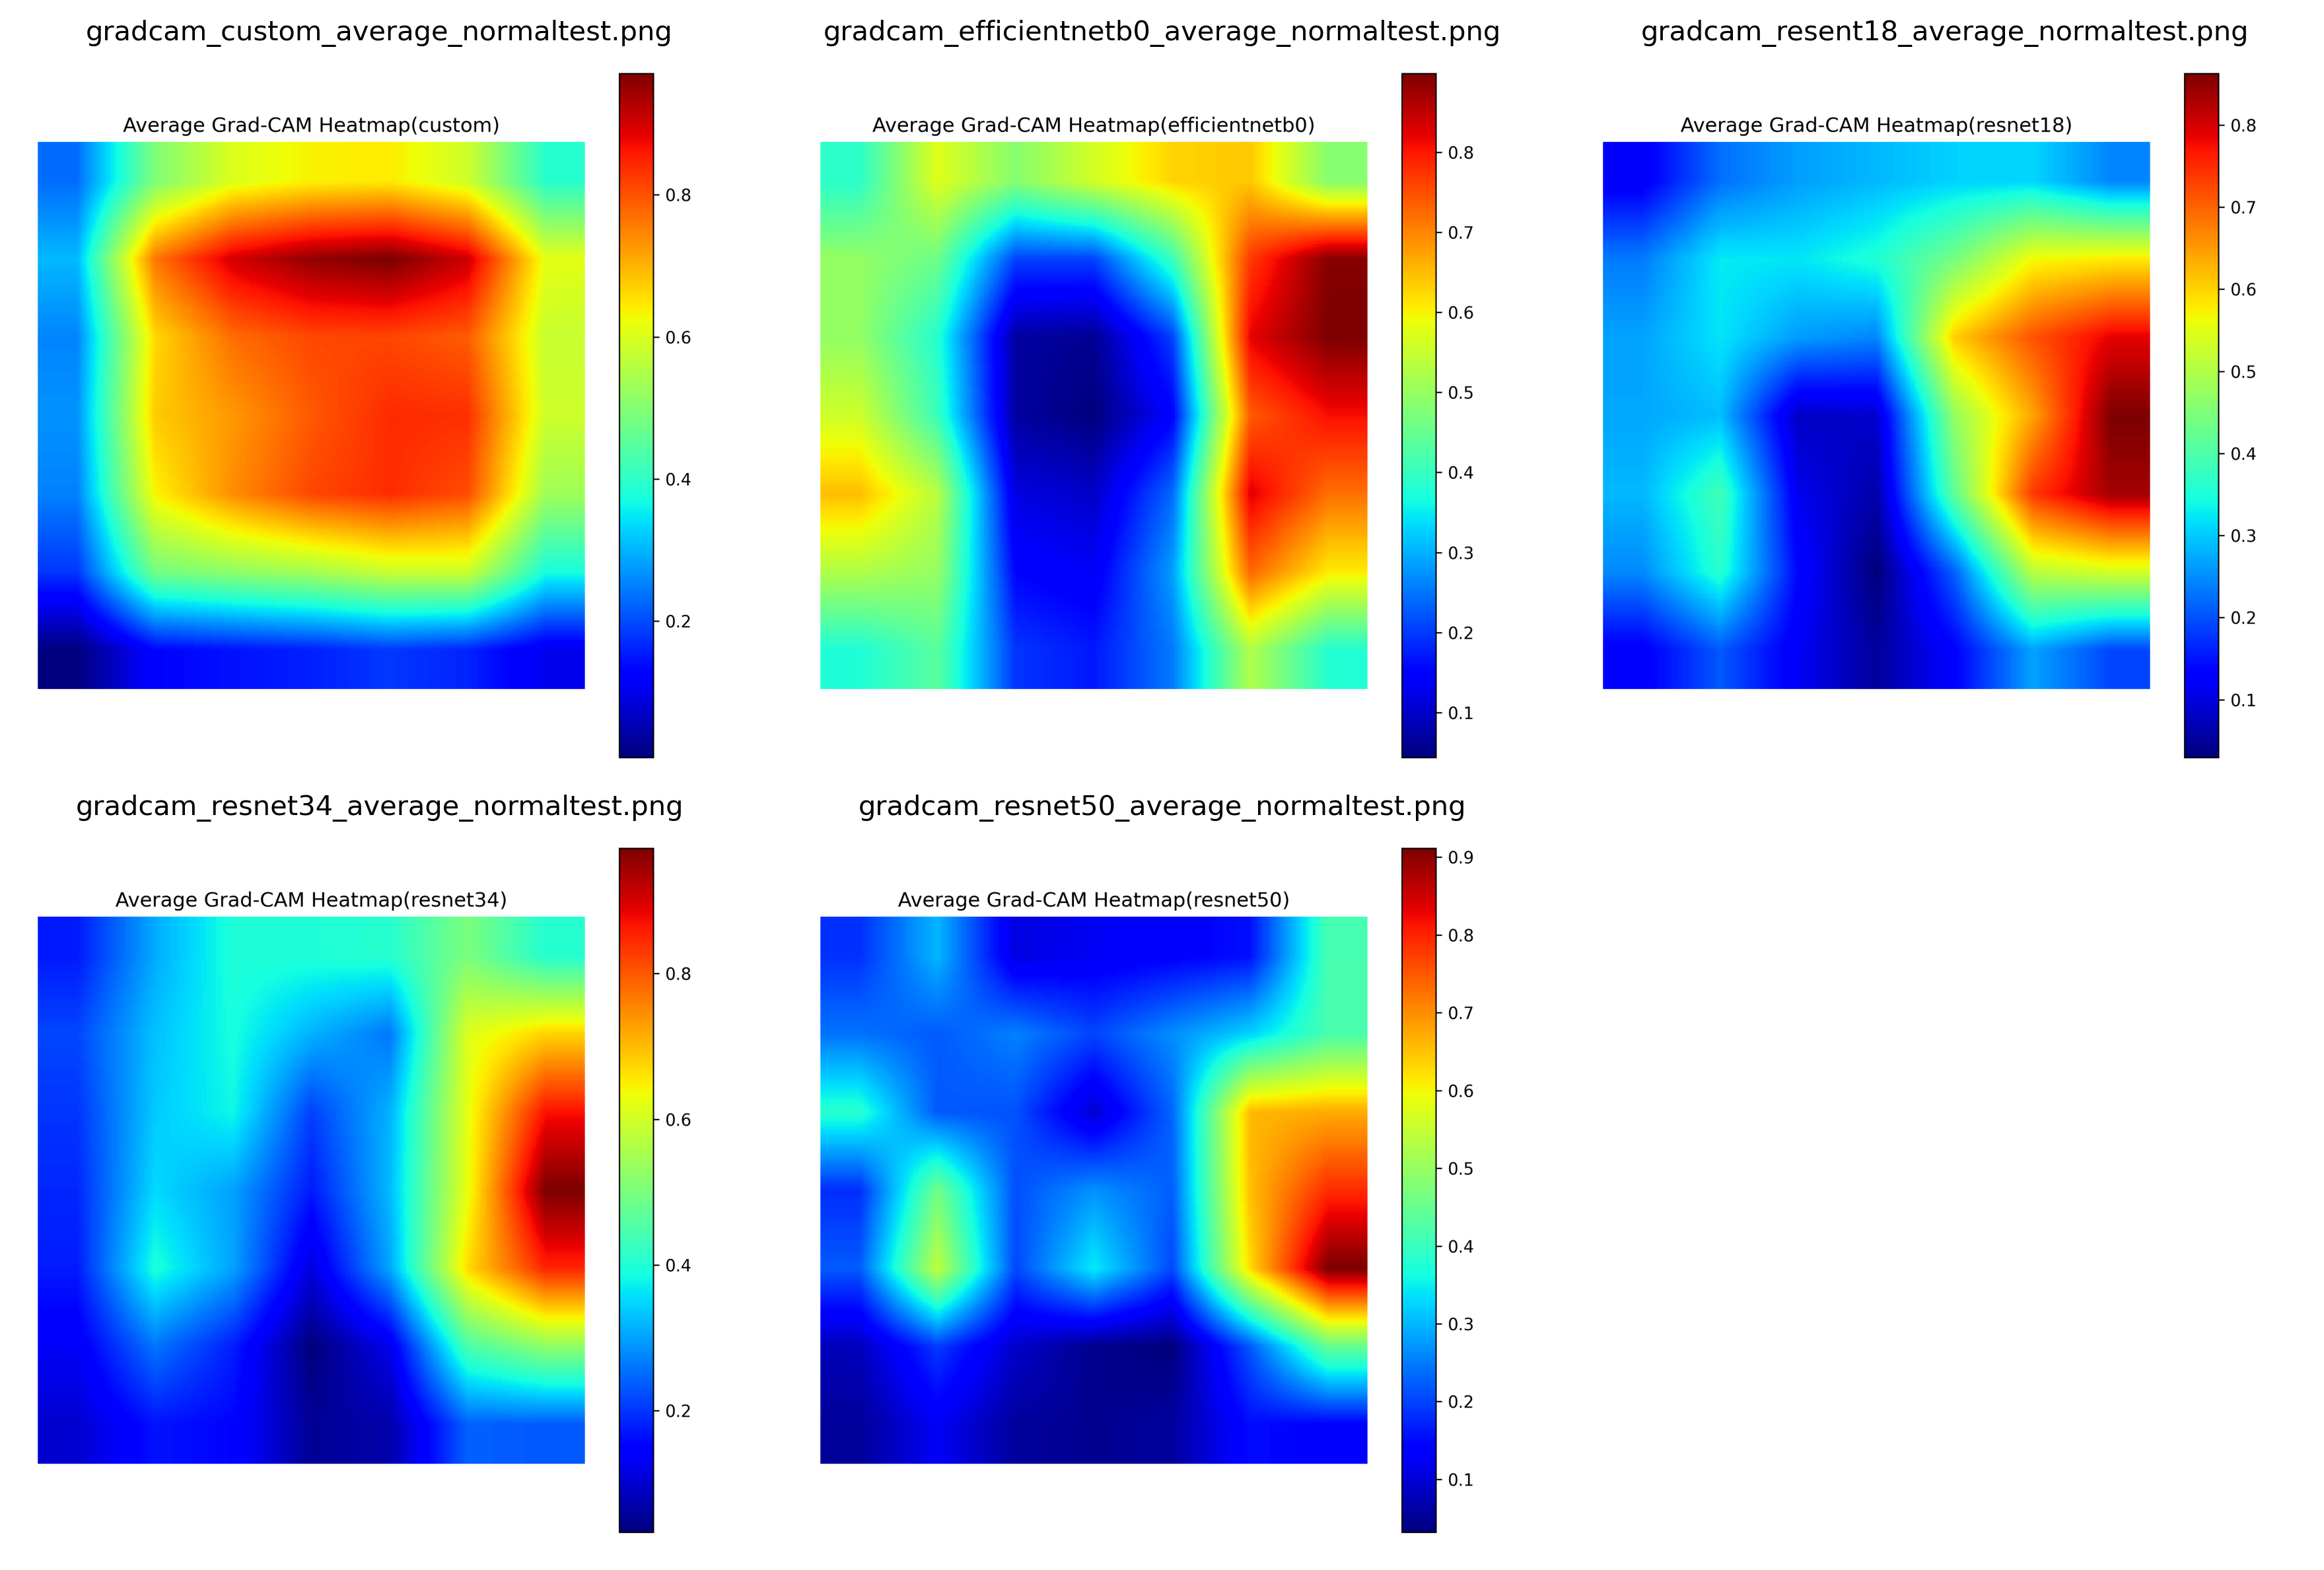
\includegraphics[width=1.1\textwidth]{combined_images_normal.png}
    \caption{Grad-CAMを用いた一般人の判断根拠の可視化}
    \label{fig:gradcam_normal}
\end{figure}
%======================

\subsubsection{検証結果の考察}
美男美女の判断根拠について,Customは顔全体,特に口元がよく見られているが,それ以外のResNet・EfficientNetについては,全体の傾向として,目と口が判断根拠になっていることがわかる。\par
一方,一般人の判断根拠について,Customモデルは目元の上部(額と思われる)を見ており,それ以外のモデルは人物の右背景を見ていることがわかる。右背景を見ているのでは目的であった顔を見て分類する目的を果たせておらず,実験の目標は達成できていない。そこで次の章では,これらの背景の影響を抑えるために画像を白背景にして再度を学習を行った。
%ただし,用意したデータセットをモデルごとに実行し,Grad-Camで得た出力の「モデルごとの平均」であることに注意したい。



\clearpage

\subsection{白背景画像を用いたGrad-Camの改善}
\subsubsection{検証の概要}

背景情報への依存を低減させる試みとして全画像の背景を白色に加工し,再度学習を行なった。
図\ref{fig:gradcam_good_white},図\ref{fig:gradcam_normal_white}にGrad-CAMを用いてモデルごとに美男美女(good)と一般人(normal)の各データの平均したヒートマップを示す。

各画像は以下に示すモデルを適用した結果である。
\begin{itemize}
	\item 1行目
	\begin{itemize}
	\item 追加学習したモデル:Custom
	\item EfficientNet\_b0
	\item ResNet18
	\end{itemize}
	\item 2行目
	\begin{itemize}
	\item ResNet34
	\item ResNet50
	\end{itemize}
\end{itemize}


\subsubsection{検証結果}
%======================
\begin{figure}[H]
    \centering
    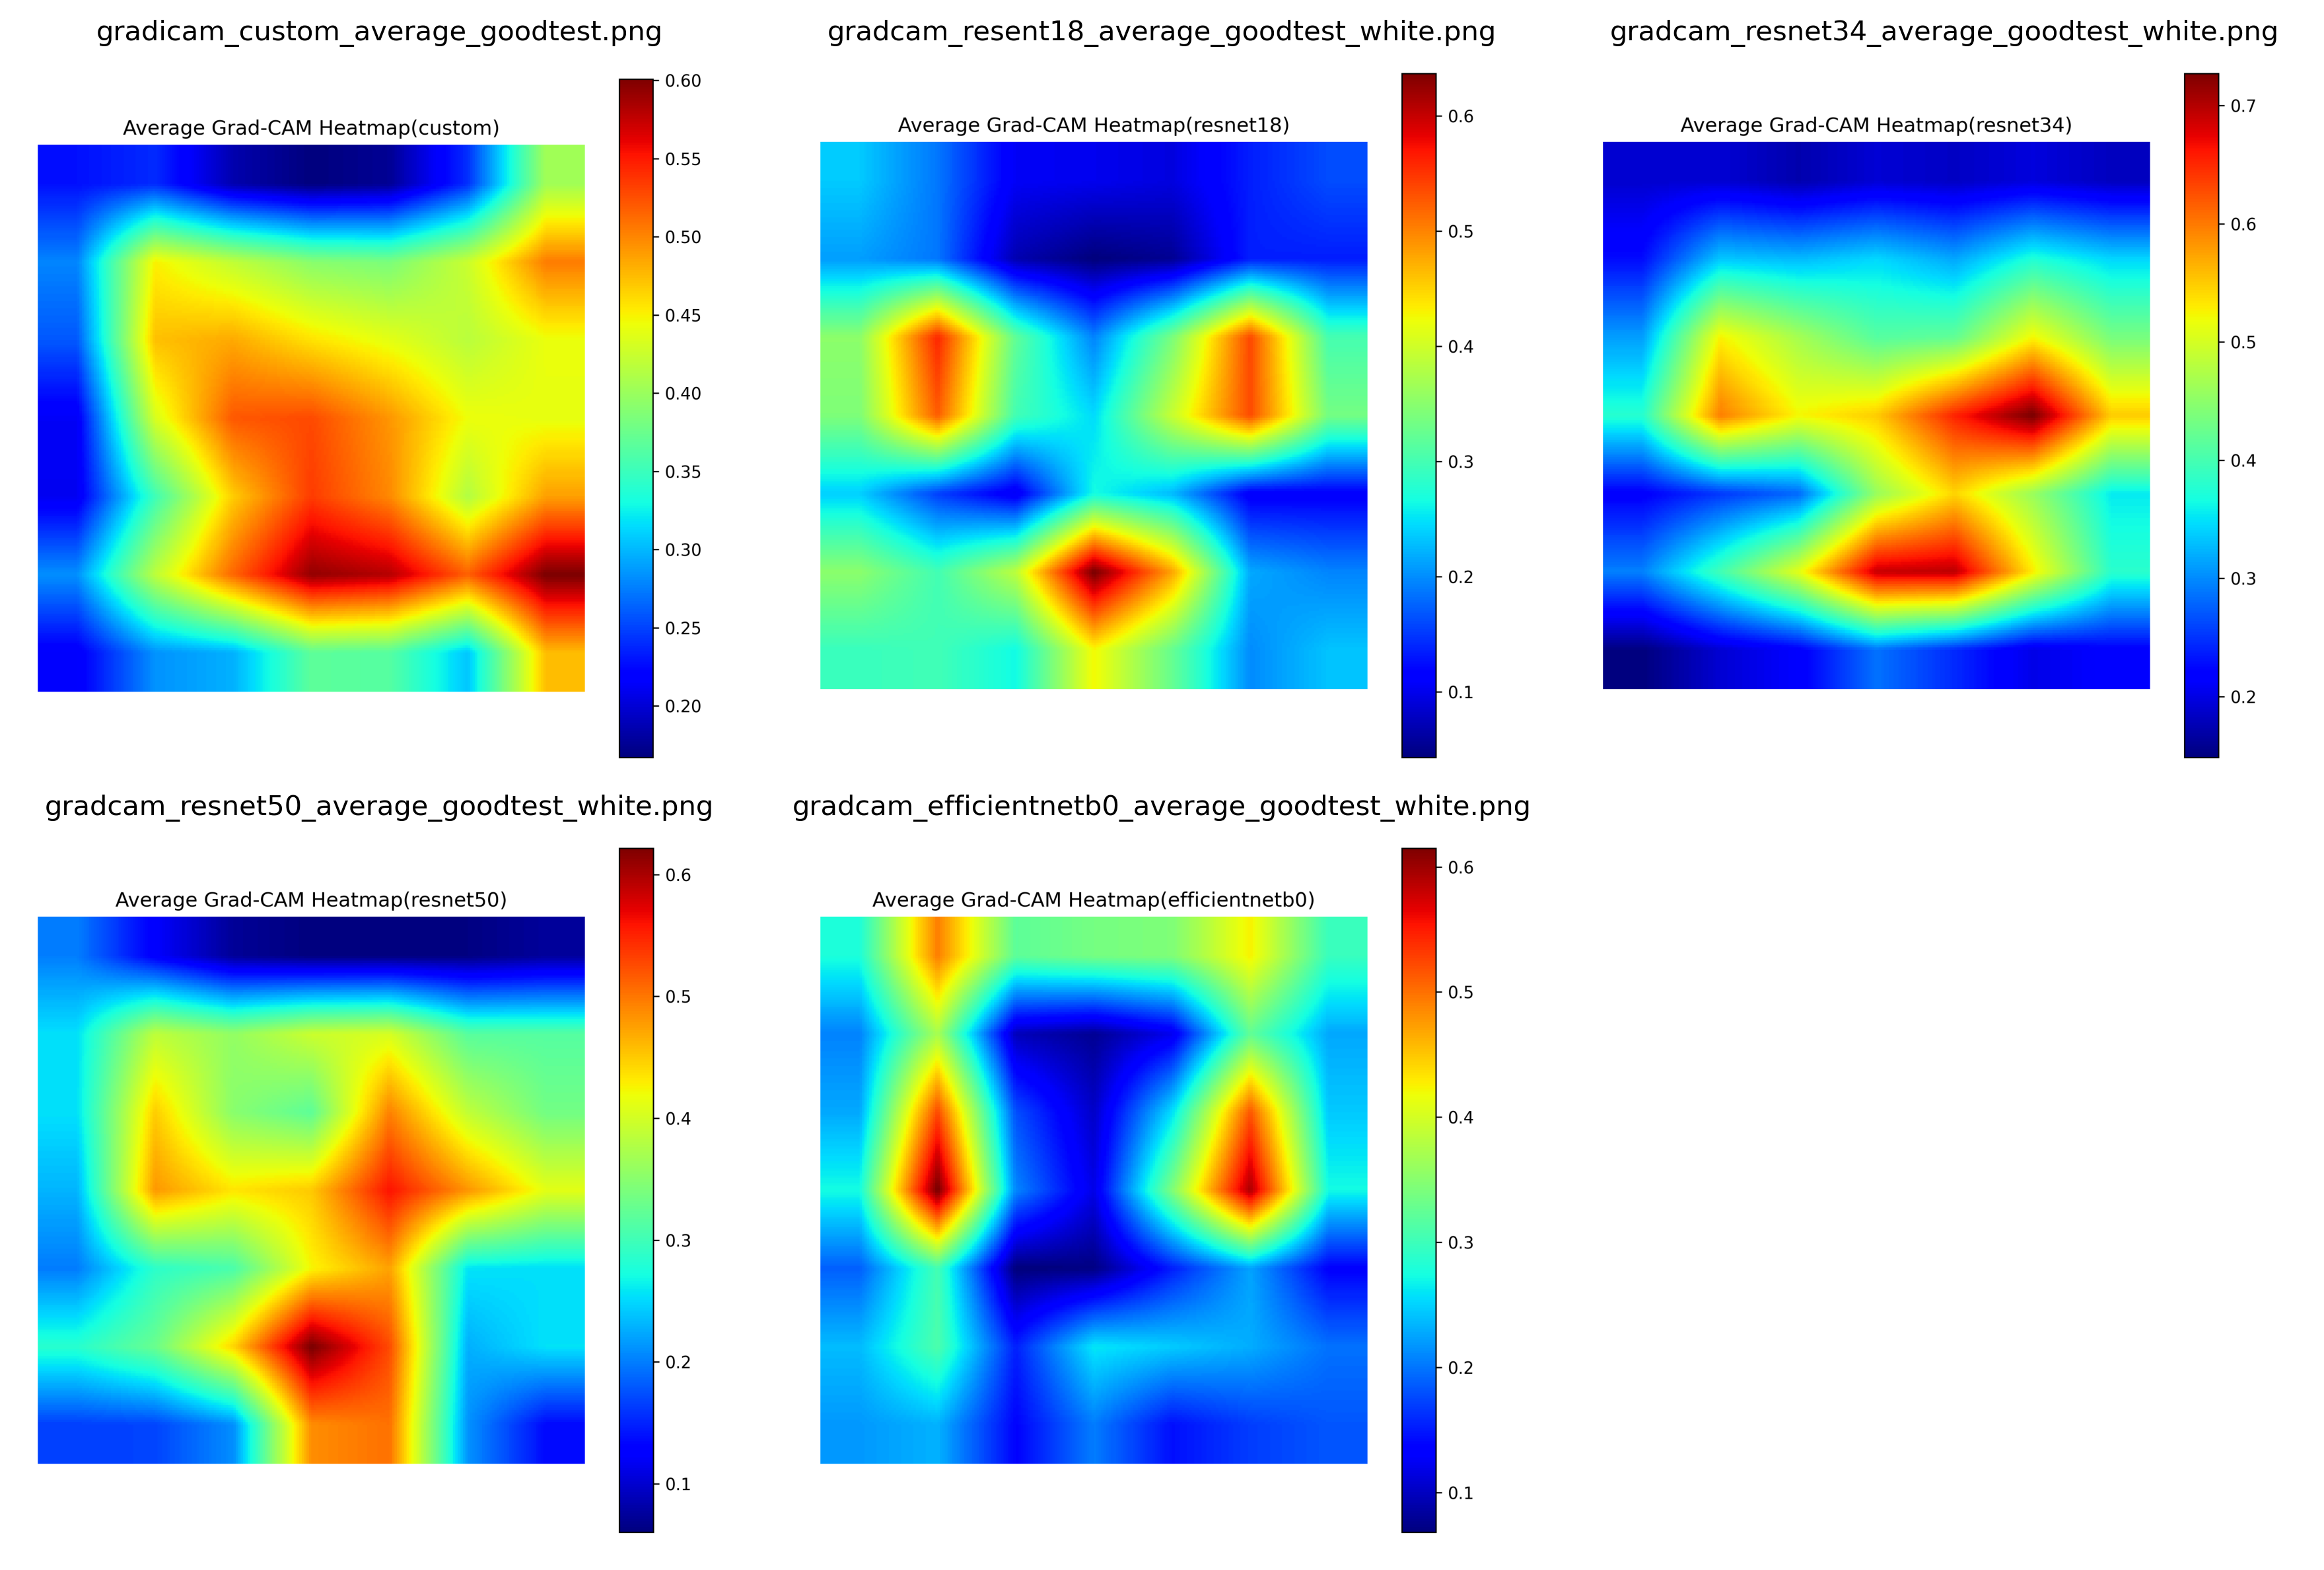
\includegraphics[width=1.1\textwidth]{white_combined_images_good.png}
    \caption{白背景でのGrad-CAMを用いた美男美女の判断根拠の可視化}
    \label{fig:gradcam_good_white}
\end{figure}
%======================
%======================
\begin{figure}[H]
    \centering
    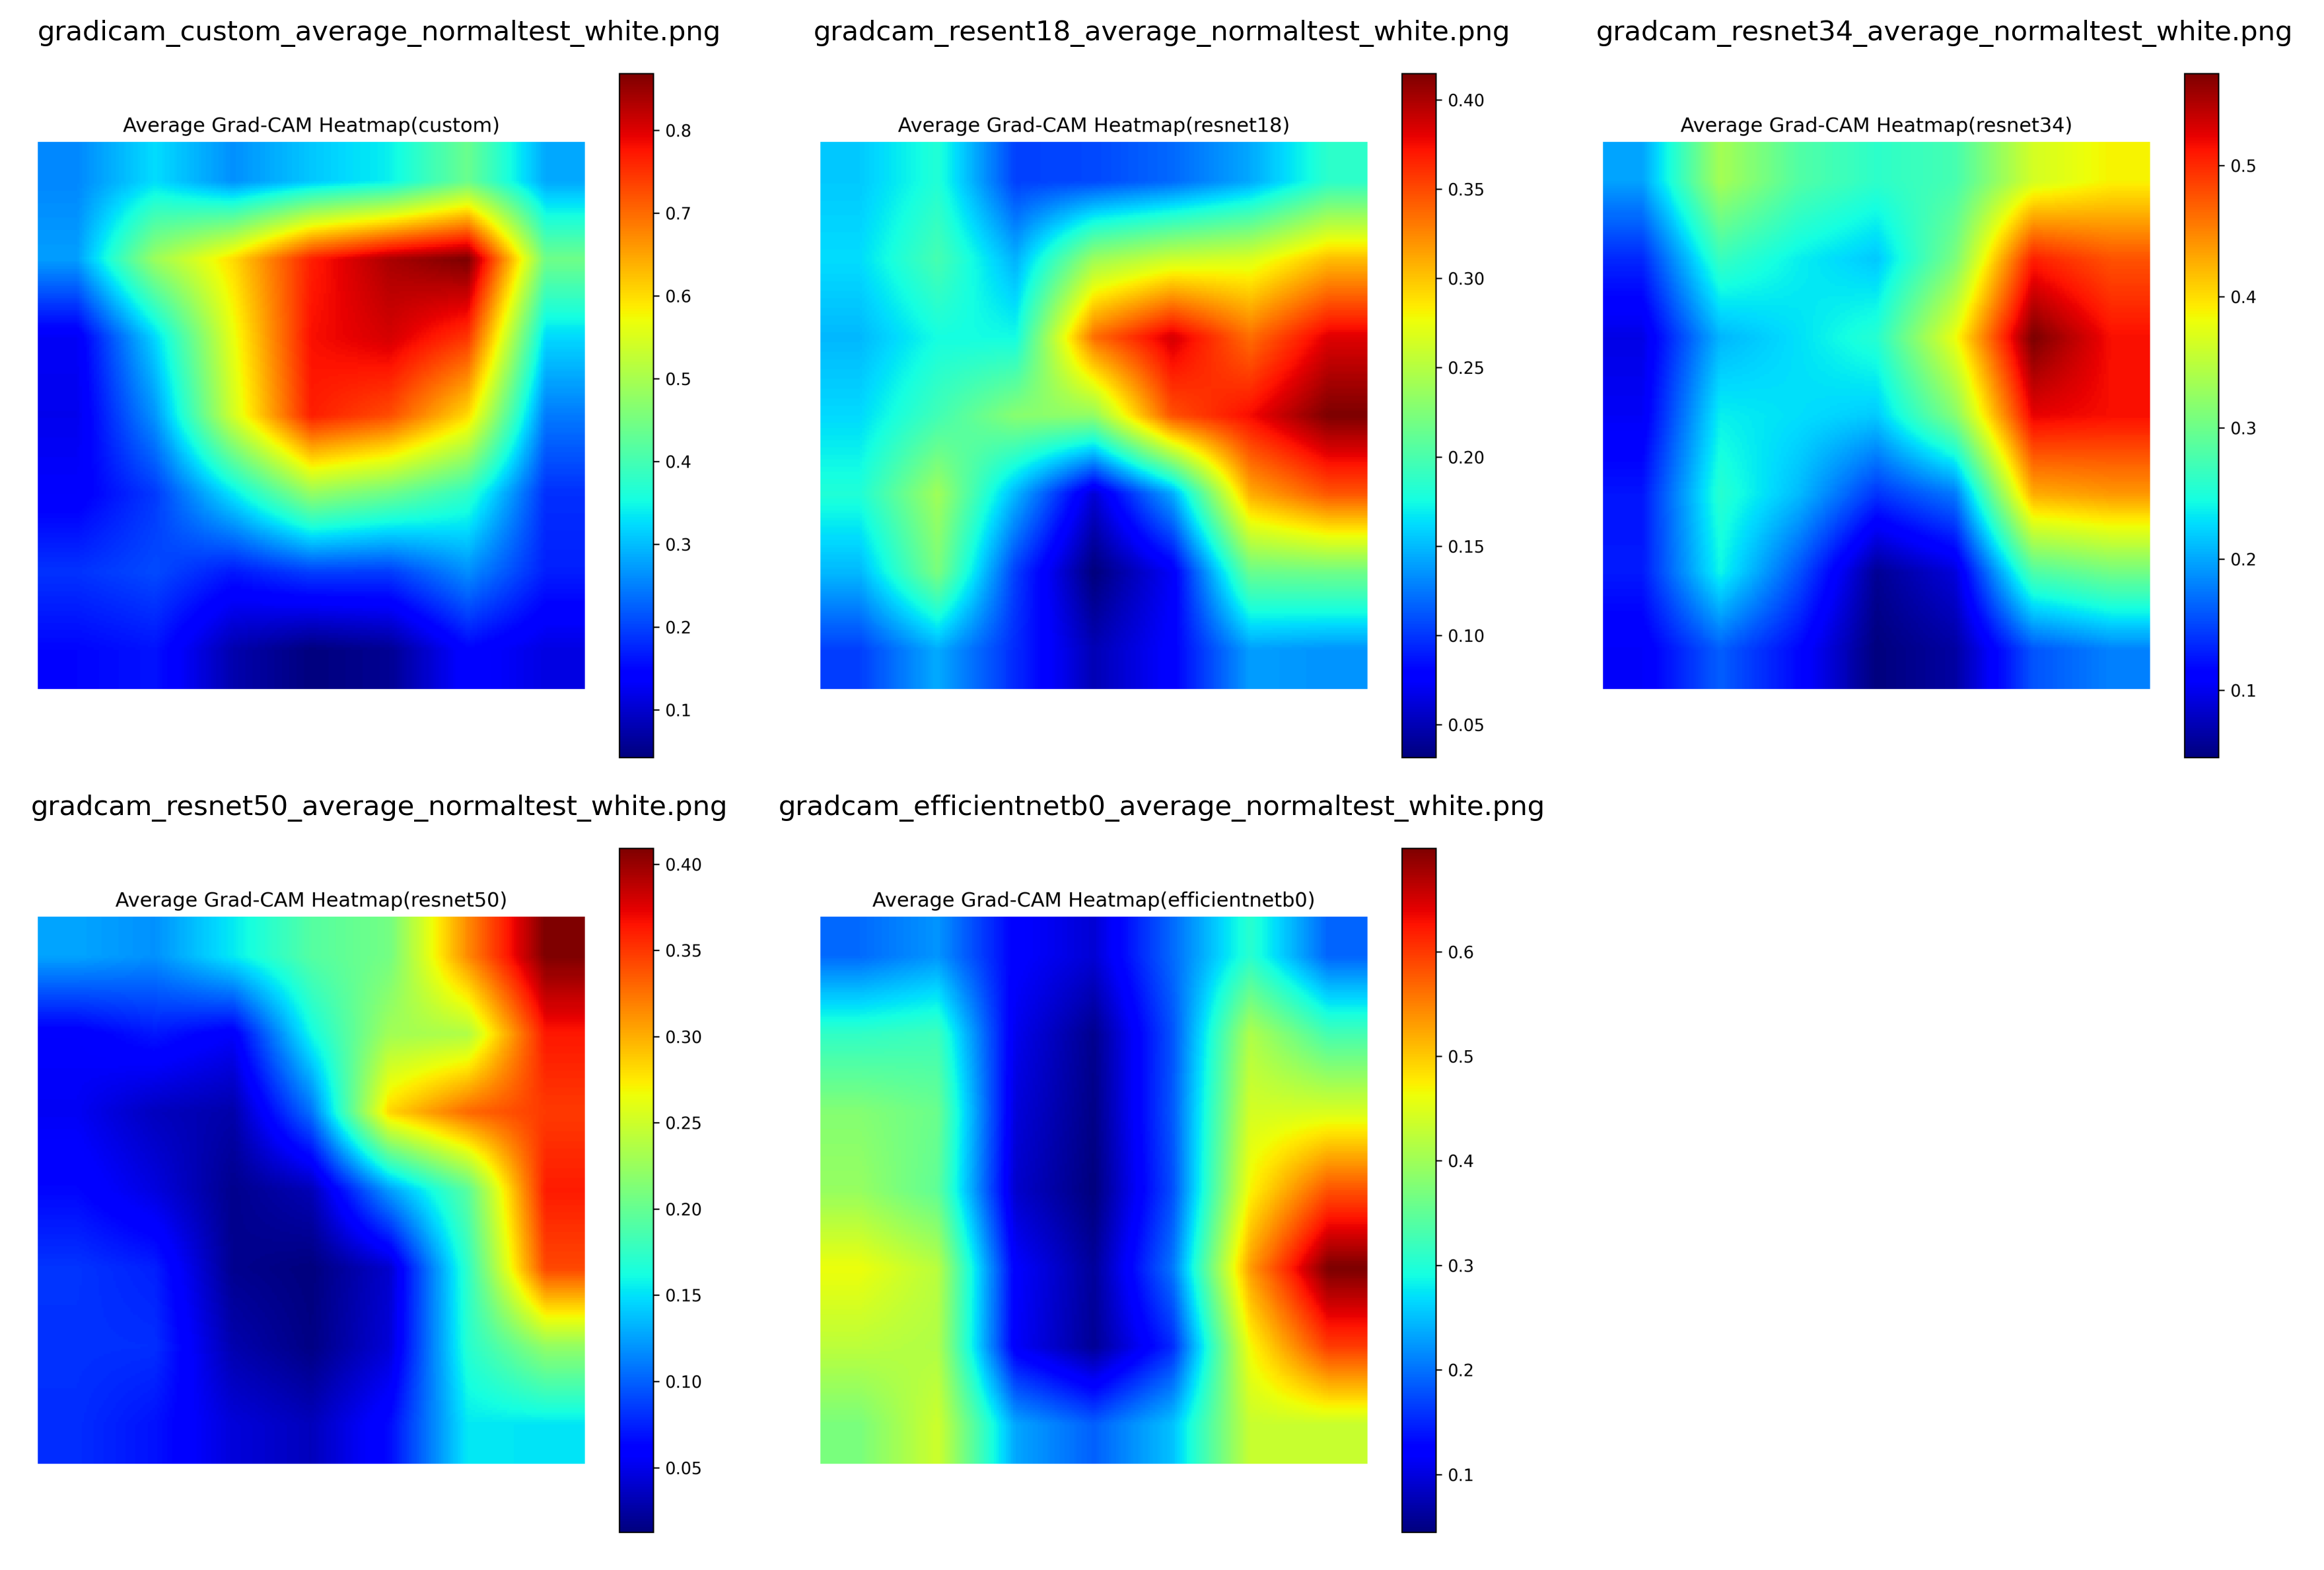
\includegraphics[width=1.1\textwidth]{white_combined_images_normal.png}
    \caption{白背景でのGrad-CAMを用いた一般人の判断根拠の可視化}
    \label{fig:gradcam_normal_white}
\end{figure}
%======================


\subsection{検証結果・考察}
\label{label:検証結果・考察}

美男美女の判断根拠については,先ほどと同様に顔全体,特に目元・口元がよく見られているが,EfficientNetについては,顔から離れた背景ないしは目元を注視している。
一方,一般人の判断根拠について,白背景の有無に関わらず右背景を注視する傾向にあり,人物には注目できていないことがわかる。
%ただし,用意したデータセットをモデルごとに実行し,Grad-Camで得た出力の「モデルごとの平均」であることに注意したい。

この原因については,データに内在していたバイアスの影響が考えられる。\par
図\ref{fig:good_ex},図\ref{fig:normal_ex}に示したように美男美女の画像の全体的な傾向として,記者会見などで用いられるバックパネルやスタジオで撮影されていると思われる画像など,背景がシンプルなものが多い。また人物の写りがよくなるように画像加工されていたり,美男美女の写真はいわゆる一眼レフなどの良いカメラが使われていたりといった可能性も考えられる。美男美女・一般人ともに$300 \times 300$にリサイズ処理を施したため,解像度については統一されているが,色やボケ感・特定の構図についてはデータセット構築時に考慮していない。\\

一方で,一般人の画像は,Flickr 画像とTwitterやオンライン新聞の画像などがデータセットに使われており,人物の横に他の人の体の一部が写っているなどの背景が乱雑なものやカメラを向いていなかったりするものが多い傾向にある。そういった構築したデータセットの画像の特徴から,一般人の分類において背景で判断されたと考えられる。\par



しかし,それを踏まえたとしてもCustom Modelは正しく顔を捉えることができており,これは『新規学習モデルが背景に注目した一方,Custom Modelが一貫して顔領域に注目できた』という事実より,FairFaceの膨大な事前学習が原因であると考察される。
また,\ref{label:仮設立て}で示した仮説による影響が考えられる。つまり,本タスクに対してResNet34であれば十分な表現能力があり,FairFaceの事前学習によって獲得された汎用的な顔特徴表現が,本タスクの学習を極めて効率的にしたと考えられる。



\section{まとめ}
\label{label:まとめ}

本実験では追加学習として美男美女・一般人の分類を行い,GradCamの結果からも顔を正しく識別しながら精度が100\%を達成していることがわかった。美男美女と称される人と一般人の差異は口もとと目が大きな影響を与えることが図\ref{fig:gradcam_good},図\ref{fig:gradcam_normal}より示唆される。



しかしながら,一般人データセットの持つ乱雑な背景や美男美女データセットのもつ背景がシンプルかつ特定の構図などのデータセットとして根本的なバイアスの影響が見られ,新規学習モデルではモデルが顔ではなく背景を判断根拠としたモデル構築となってしまった。白背景に加工し再度GradCamを実行しても,一般人の判断根拠について,白背景の有無に関わらず右背景を注視する傾向にあり,人物には注目できていない点は変わらなかった。

新規学習において,バイアスをモデルが捉えている可能性があり,データセットそのもの自体の欠如を示唆している。Custom Modelが高精度であったのは,事前学習によって顔領域を正しく認識できているためと考えられる。


\section{反省・今後の課題}

\subsection{反省点}
\subsubsection*{データセットの誤り}
新規学習モデルと追加学習モデルとの比較によって,構築したデータセットに誤りが含まれていることがあきらかになった。まとめると,以下のバイアスが構築したデータセットに含まれると考えられる。
\begin{itemize}
	\item 一般人データセットの再利用の影響
		\begin{itemize}
			\item \textbf{想定される対処:}有名人データセット同様に一般人データセットを独自構築する。
		\end{itemize}
	\item  撮影日時の不均一性と年齢による特徴変化の未考慮(対処困難)
	\item 背景・撮影状況のバイアス
		\begin{itemize}
			\item \textbf{想定される対処:}白背景にしてもGradCamの一般人の結果は変化しなかったため,偏りのないデータを多く用意する必要がある。
		\end{itemize}
	\item 画像のプロパティ(色、構図)の未考慮
		\begin{itemize}
			\item \textbf{想定される対処:}グレイスケールにする,顔のみ切り抜くなど
		\end{itemize}
\end{itemize}

\subsubsection*{実験計画の見積もりミス}
当初の調べ不足が原因でFairFaceがデータセットのみを公開していると認識してしまっており,実験にかけられる時間が少なくなってしまった。また,実験計画よりも前処理に時間がかかり、その後の実行と結果考察のための時間が不足してしまった。

\subsubsection*{プロジェクト管理の欠如}
GitHubを使おうとしたが,使える人数が少なくGitHubでのバージョン管理が実質できていなかった。さらにamaneで実行する場合,さらにソースコードのバージョンが不透明になってしまった。
役割分担・実験計画が適切にできておらず,実験の後半で急いで学習を行った。計画よりも前処理に時間がかかり,その後も実行しその結果を考察する時間をファイルの欠損の対応・コンテナプラットフォームSingularity使用のための準備といった対応に終われてしまった。

%==============================
\subsection{時間の都合上省いた項目}
\subsubsection*{撮影日時による人物データの抽出}
画像をwebスクレイピングで収集したものについて,ネットに存在する美男美女の画像は撮影された日時がバラバラである。若い時の写真もあれば現在の写真もあり,年齢によって発生する特徴量の変化については考慮できていない。検索キーワードをもとにスクレイピングをする際に,人名に年齢を含むアプローチも行ったが,得られる画像が少ない・検索してもそもそも年齢で絞れないという課題が生じた。本実験で調べる限りは実験の限界と判断し,他の前処理を丁寧に行う方を優先した。

\subsubsection*{構築したデータセットの人名の偏り改善}
本実験では,2024年美男美女ランキングtop50をもとに,50名ずつ抽出し,アップサンプリング(左右反転)を施した。これは一般人のデータセットと比較して,偏りが生じる。他のアップサンプリングの方法として回転・輝度変更といった手法があるが,これらでさらにデータを増やすよりかは,美男美女の人名数を50名ずつよりさらに増やす方がバイアスを削減できると考える。本実験では時間の都合・第一回の実験時の計画がずれていたため省略した。




\begin{thebibliography}{9}
    \bibitem{karkkainenFairFace}
    Karkkainen, Kimmo and Joo, Jungseock.
    FairFace: Face Attribute Dataset for Balanced Race, Gender, and Age for Bias Measurement and Mitigation.
    In \textit{Proceedings of the IEEE/CVF Winter Conference on Applications of Computer Vision}, pages 1548--1558, 2021.\\
        \url{https://arxiv.org/abs/1908.04913}
    
    \bibitem{bidanshi}
    Most Handsome Man In The World 2024, shiningawards.com, \\
    \url{https://shiningawards.com/most-handsome-man-in-the-world-2024/}
    
    \bibitem{bijoshi}
    Most Beautiful Faces 2024, gigazine.net, \\ \url{https://gigazine.net/gsc_news/en/20241229-most-beautiful-faces-2024/}
    
        \bibitem{hopenet_paper}
        Nataniel Ruiz Eunji Chong and James M. Rehg (Georgia Institute of Technology).
        Fine-Grained Head Pose Estimation Without Keypoints
         In \textit{The IEEE Conference on Computer Vision and Pattern Recognition (CVPR) Workshops}, pages 2074--2083, 2018. \\
          \url{https://arxiv.org/abs/1710.00925}

    \bibitem{hopenet}
    Head Pose Estimation, \url{https://github.com/natanielruiz/deep-head-pose}
    \bibitem{gradcam}Grad-CAM: Visual Explanations from Deep Networks via Gradient-based Localization, 
    Ramprasaath R. Selvaraju, Michael Cogswell, Abhishek Das, Ramakrishna Vedantam, Devi Parikh, Dhruv Batra,\\
    \url{https://arxiv.org/abs/1610.02391}
    
  %github repo: https://github.com/jacobgil/pytorch-grad-cam
\end{thebibliography}


% ==============================================================================
\clearpage
\appendix % 付録部分の始まり
\section{GradCamを用いた分析の詳細}

\subsection{GradCamを用いた分析の実行結果}

図\ref{fig:append_custom(good)}にCustom Model (good),
図\ref{fig:append_custom(normal)}にCustom Model (normal),
図\ref{fig:append_efficientnetb0(good)}にEfficientNetB0 (good),
図\ref{fig:append_efficientnetb0(normal)}にEfficientNetB0 (normal),
図\ref{fig:append_resent18(good)}にResNet18 (good),
図\ref{fig:append_resnet18(normal)}にResNet18 (normal),
図\ref{fig:append_resnet34(good)}にResNet34 (good),
図\ref{fig:append_resnet34(normal)}にResNet34 (normal),
図\ref{fig:append_resnet50(good)}にResNet50 (good),
図\ref{fig:append_resnet50(normal)}にResNet50 (normal) の実行結果を示す。
これらは,構築したデータセットの画像に対してGradCamのヒートマップを描画したものであり,客観的にモデルが顔領域のどの部分をみているのかを示す。

% Custom(good)
\begin{figure}[H]
    \centering
    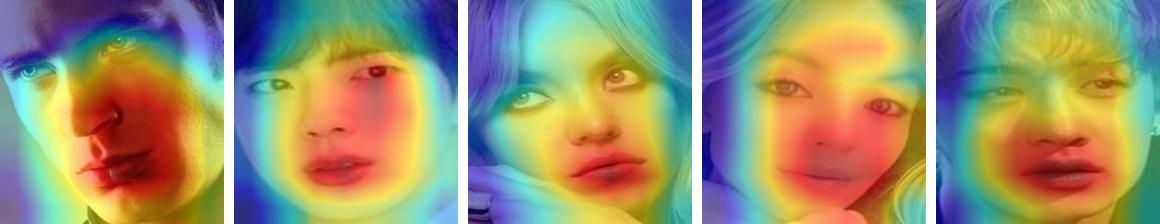
\includegraphics[width=1.1\textwidth]{custom(good).jpg}
    \caption{Custom Model (good) の実行結果}
    \label{fig:append_custom(good)}
\end{figure}

% Custom(normal)
\begin{figure}[H]
    \centering
    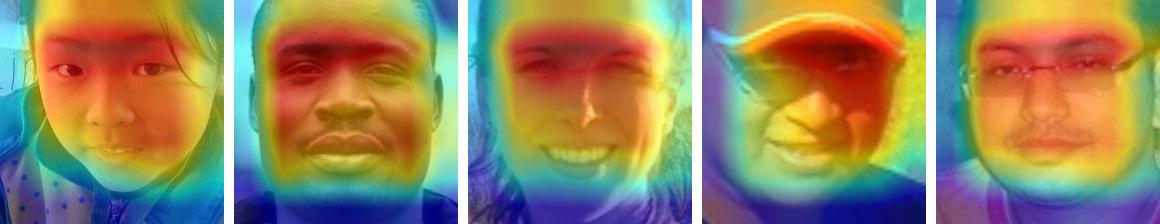
\includegraphics[width=1.1\textwidth]{custom(normal).jpg}
    \caption{Custom Model (normal) の実行結果}
    \label{fig:append_custom(normal)}
\end{figure}

% EfficientNetB0(good)
\begin{figure}[H]
    \centering
    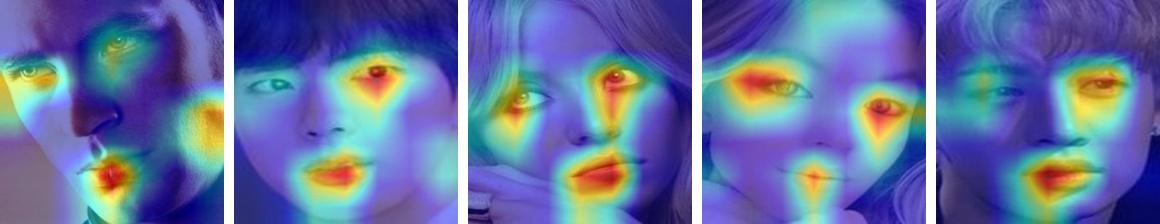
\includegraphics[width=1.1\textwidth]{efficientnetb0(good).jpg}
    \caption{EfficientNetB0 (good) の実行結果}
    \label{fig:append_efficientnetb0(good)}
\end{figure}

% EfficientNetB0(normal)
\begin{figure}[H]
    \centering
    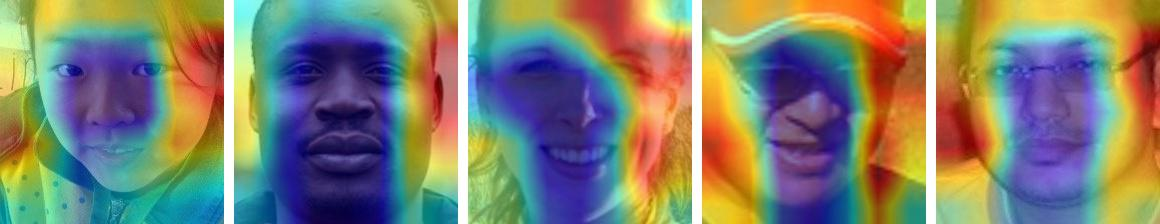
\includegraphics[width=1.1\textwidth]{efficientnetb0(normal).jpg}
    \caption{EfficientNetB0 (normal) の実行結果}
    \label{fig:append_efficientnetb0(normal)}
\end{figure}

% ResNet18(good)
\begin{figure}[H]
    \centering
    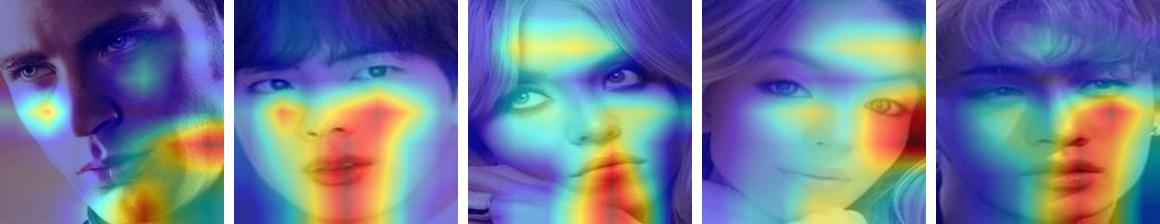
\includegraphics[width=1.1\textwidth]{resent18(good).jpg}
    \caption{ResNet18 (good) の実行結果}
    \label{fig:append_resent18(good)}
\end{figure}

% ResNet18(normal)
\begin{figure}[H]
    \centering
    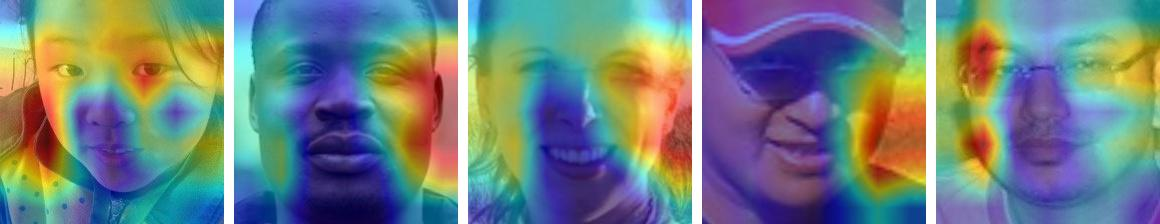
\includegraphics[width=1.1\textwidth]{resnet18(normal).jpg}
    \caption{ResNet18 (normal) の実行結果}
    \label{fig:append_resnet18(normal)}
\end{figure}

% ResNet34(good)
\begin{figure}[H]
    \centering
    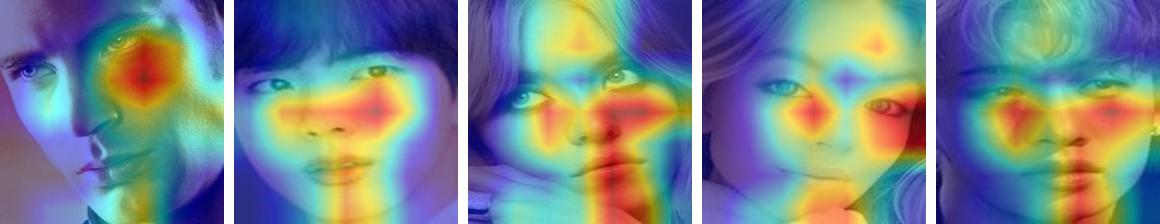
\includegraphics[width=1.1\textwidth]{resnet34(good).jpg}
    \caption{ResNet34 (good) の実行結果}
    \label{fig:append_resnet34(good)}
\end{figure}

% ResNet34(normal)
\begin{figure}[H]
    \centering
    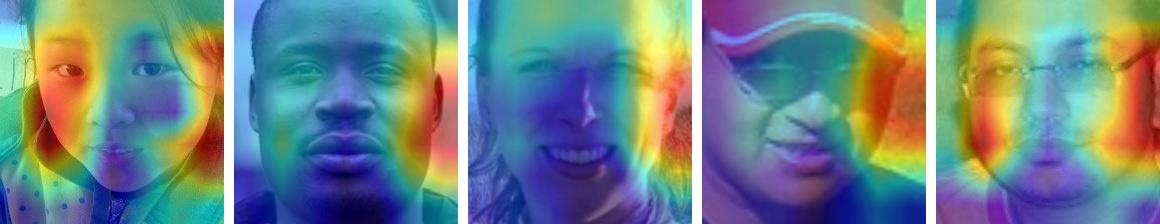
\includegraphics[width=1.1\textwidth]{resnet34(normal).jpg}
    \caption{ResNet34 (normal) の実行結果}
    \label{fig:append_resnet34(normal)}
\end{figure}

% ResNet50(good)
\begin{figure}[H]
    \centering
    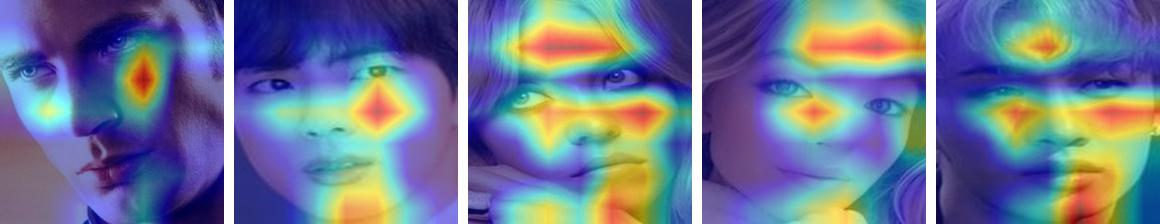
\includegraphics[width=1.1\textwidth]{resnet50(good).jpg}
    \caption{ResNet50 (good) の実行結果}
    \label{fig:append_resnet50(good)}
\end{figure}

% ResNet50(normal)
\begin{figure}[H]
    \centering
    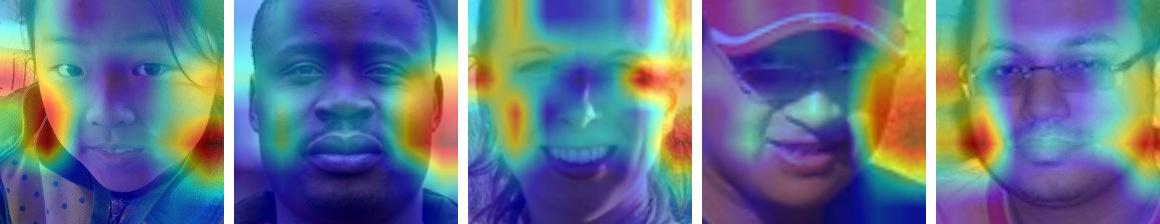
\includegraphics[width=1.1\textwidth]{resnet50(normal).jpg}
    \caption{ResNet50 (normal) の実行結果}
    \label{fig:append_resnet50(normal)}
\end{figure}


\subsection{考察}
全体的な傾向として,美男美女の顔画像では,モデルの注目は目,鼻,口といった顔の中心的なパーツに強く集中している一方で,一般人の画像では注目領域が頬,額,顎の輪郭,背景など拡散している傾向が見られる。判断の根拠となる明確な特徴を見つけられていないことがわかる。


図\ref{fig:append_custom(good)}では,両目,鼻,口といった顔の中心領域をバランスよく見ていることがわかる。特定の偏りが見られていない。図\ref{fig:append_custom(normal)}では,額付近を注視している傾向にあるが,顔の輪郭全体から特徴を見ていることがわかる。\par
図\ref{fig:append_efficientnetb0(good)}では,実行したモデルの中で最も目元を注目しているといえる。一方で,一般人(図\ref{fig:append_efficientnetb0(normal)})ではそのような傾向が見られず背景や衣服を見て判断していることがわかる。\par

図\ref{fig:append_resent18(good)}では,顔の特に口元を注視する傾向にあり,図\ref{fig:append_resnet18(normal)}は右背景や目元付近を学習している傾向にある。\par
図\ref{fig:append_resnet34(good)}では,目・鼻・口を注目しており,図\ref{fig:append_custom(good)}と同じような傾向が伺える。一方で,図\ref{fig:append_resnet34(normal)}は背景を特に注目している。\par

図\ref{fig:append_resnet50(good)}は注目領域がシャープになっており,頬や額を見て判断している傾向にあるが,図\ref{fig:append_resnet50(normal)}では依然として背景を見て判断してしまっている。

\end{document}
